\documentclass[UTF8]{ctexart}
\newcommand{\mycmdB}[1]{{\heiti #1}}
\renewcommand{\normalsize}{\fontsize{12}{12}\fangsong}
\usepackage{listings}
\usepackage{xcolor}
\usepackage{amsmath}
\usepackage{graphicx} 
\usepackage{float} 
\usepackage{indentfirst}
\usepackage{longtable}
\usepackage{fancyhdr}
\usepackage[a4paper, left=2.5cm, right=2.5cm, top=3cm, bottom=2cm]{geometry}
\usepackage{matlab-prettifier}
\usepackage{latexcolors}

\setlength{\parindent}{2em} %2em代表首行缩进2个字符

% 页眉页脚设置
\pagestyle{fancy}
\fancyhf{}
\lhead{2021300045}
\chead{李宗霖}
\rhead{第\thepage 页}

% 去除图注冒号
\usepackage{caption}
\captionsetup[table]{labelsep=space} % 表
\captionsetup[figure]{labelsep=space} % 图 

\CTEXsetup[format={\Large\bfseries}]{section}

% 源代码引用
\renewcommand{\lstlistingname}{源代码}
\lstset{
    basicstyle          =   \zihao{5} \ttfamily,          % 基本代码风格
    keywordstyle        =   \bfseries,          % 关键字风格
    commentstyle        =   \ttfamily\itshape,  % 注释的风格,斜体
    stringstyle         =   \ttfamily,  % 字符串风格
    flexiblecolumns,                % 别问为什么,加上这个
    numbers             =   left,   % 行号的位置在左边
    showspaces          =   false,  % 是否显示空格,显示了有点乱,所以不现实了
    numberstyle         =   \zihao{5}\ttfamily,    % 行号的样式,小五号,tt等宽字体
    showstringspaces    =   false,
    captionpos          =   t,      % 这段代码的名字所呈现的位置,t指的是top上面,b指下面
    frame               =   lrtb %lrtb,   % 显示边框
}
\lstset{
	language            = matlab,
    basicstyle          = \zihao{5}\ttfamily,          % 基本代码风格
	rulesepcolor        = \color{gray}, % 代码块边框颜色
	breaklines          = true, % 代码过长则换行
	numbers             = left, % 行号在左侧显示
	numberstyle         = \zihao{5}\ttfamily,  % 行号字体
	showspaces          = false, % 不显示空格
	columns             = fixed, % 字间距固定
	%morekeywords        = {as}, % 自加新的关键字(必须前后都是空格)
	%deletendkeywords    = {compile} % 删除内定关键字;删除错误标记的关键字用deletekeywords删!
}

\lstdefinestyle{Python}{
    language        =   Python, % 语言选Python
    basicstyle      =   \zihao{5}\ttfamily,
    numberstyle     =   \zihao{5}\ttfamily,
    keywordstyle    =   \color{blue},
    keywordstyle    =   [2] \color{teal},
    stringstyle     =   \color{magenta},
    commentstyle    =   \color{red}\ttfamily,
    breaklines      =   true,   % 自动换行,建议不要写太长的行
    columns         =   fixed,  % 如果不加这一句,字间距就不固定,很丑,必须加
    basewidth       =   0.5em,
}

\begin{document}

\begin{center}
    {\zihao{-2} \bf 航天飞行动力学}\\
    {\zihao{3} 第三次作业\ ——\ 飞行方案设计}

\end{center}

\section*{\zihao{-4} 一、题目}
\noindent {\heiti 1.导弹参数:}

\begin{itemize}
    \item[*] 导弹质量$m_0=320kg$
    \item[*] 发动机推力$P=2000N$
    \item[*] 初始速度$V_0=250m/s$
    \item[*] 初始位置$x_0=0m$
    \item[*] 初始高度$H_0=7000m$
    \item[*] 初始弹道倾角$\theta=0^{\circ}$
    \item[*] 初始俯仰角 $\varphi_0=0^\circ$
    \item[*] 初始攻角 $\alpha_0=0^\circ$
    \item[*] 初始俯仰角速度$\dot{\varphi}_0=0rad$/s
    \item[*] 初始速度$V_0=250m/s$
    \item[*] 参考长度$S_{ref}=0.45 m^{2}$
    \item[*] 参考面积$L_{ref}=2.5m$
    \item[*] 升力系数$C_{y}=0.25\alpha+0.05\delta_{z}$
    \item[*] 阻力系数$C_x=0.2+0.005\alpha^2$
    \item[*] 俯仰力矩系数$m_z=-0.1\alpha+0.024\delta_z$
\end{itemize}

\noindent {\heiti 2.大气密度计算公式:}
\begin{align}
    \begin{cases}
        \rho_0=1.2495\ kg/m^3 \\
        T_0=288.15   K        \\
        T=T_0-0.0065H         \\
        \rho=\rho_{0}\left( \frac{T}{T_{0}} \right)^{4.25588}
    \end{cases}
\end{align}

\noindent {\heiti 3.飞行方案:}

\begin{itemize}
    \item[(1)] 当$x<9100m$时,采用瞬时平衡假设
        \begin{align}
            \begin{cases}
                H^*=2000\times\cos(0.000314\times1.1\times x)+5000                     \\
                \delta_z=k_\varphi\times(H\text{ -}H^*)+k_\varphi\times(H\text{ -}H^*) \\
                \delta_z=k_\varphi(H-H^*)+\dot{k}_\varphi H                            \\
                m_{s}=0.0kg/s
            \end{cases}
        \end{align}
    \item[(2)] 当$24000m>x>9100m$时,等高飞行方案,采用瞬时平衡假设。
        \begin{align}
            \begin{cases}
                H^*=3050m                                   \\
                \delta_z=k_\varphi(H-H^*)+\dot{k}_\varphi H \\
                \delta_z=k_\varphi(H-H^*)+\dot{k}_\varphi H \\
                m_s=0.46kg/s
            \end{cases}
        \end{align}
    \item[(3)] 当$x>24000m\&\&y>0$,目标位置为$x_m=30000m$,采用比例导引法和瞬时平衡假设
        \begin{align}
            \begin{cases}
                x_m=30000 m                               \\
                m_z^\alpha\alpha+m_z^{\delta_z}\delta_z=0 \\
                m_s=0.0kg/s
            \end{cases}
        \end{align}
\end{itemize}

注:舵偏角约束$\left|\delta_{z} \right|\leq 30^{\circ}$




\section*{\zihao{-4} 二、公式推导}


\noindent {\heiti 1.$x<24000m$的飞行方案:}

基于“瞬时平衡”假设,将包含20个方程的导弹运动方程组简化为铅垂平面内的质心运动方程组。
\begin{align}
    \begin{cases}
        m\frac{\mathrm{d}V}{\mathrm{d}t}=P\cos\alpha-X-mg\sin\theta\hfill                                     \\
        mV\frac{\mathrm{d}\theta}{\mathrm{d}t}=P\sin\alpha+Y-mg\cos\theta\hfill                               \\
        \frac{\mathrm{d}x}{\mathrm{d}t}=V\cos\theta \hfill                                                    \\
        \frac{dy}{dt}=V\sin\theta \hfill                                                                      \\
        \frac{dm}{dt}=-m_{s} \hfill                                                                           \\
        \alpha_b=-\frac{m_{z}^{\delta_z}}{m_{z}^{\alpha}}\delta_{zb} \hfill                                   \\
        \delta_z = k_\varphi \left(H-H^{*}\right) +\dot{k}_{\varphi} \left(\dot{H} -\dot{H}^{*}\right) \hfill \\
        H^{*}=2000\times \cos\left(0.000314\times1.1\times x\right)+5000\hfill
    \end{cases}
\end{align}

代入各物理量定义式:
\begin{align}
    \begin{cases}
        \frac{\mathrm{d}V}{\mathrm{d}t}=\frac{P\cos\alpha-X}{m}-g\sin\theta\hfill                             \\
        \frac{\mathrm{d}\theta}{\mathrm{d}t}=\frac{P\sin\alpha+Y}{m}-\frac{g\cos\theta}{V}\hfill              \\
        \frac{\mathrm{d}x}{\mathrm{d}t}=V\cos\theta \hfill                                                    \\
        \frac{dy}{dt}=V\sin\theta \hfill                                                                      \\
        \frac{dm}{dt}=-m_{s} \hfill                                                                           \\
        \alpha_b=-\frac{m_{z}^{\delta_z}}{m_{z}^{\alpha}}\delta_{zb} \hfill                                   \\
        \delta_z = k_\varphi \left(H-H^{*}\right) +\dot{k}_{\varphi} \left(\dot{H} -\dot{H}^{*}\right) \hfill \\
        H^{*}=2000\times \cos\left(0.000314\times1.1\times x\right)+5000\hfill                                \\
        Y=\left(0.25\alpha+0.05\delta_{z}\right)\times \frac{1}{2}\rho V^{2} \times S_{ref}                   \\
        X=\left(0.2+0.005\alpha^2\right)\times \frac{1}{2}\rho V^{2} \times S_{ref}
    \end{cases}
\end{align}



\noindent {\heiti 2.$x>24000m$的飞行方案:}

\noindent {(1) 末段第一种计算方法:}


\begin{align}
    \begin{cases}
        r\frac{dq}{dt}=V_{m}\times\sin\eta-V_{T}\sin\eta_{T} \\
        \tan q=\frac{y_{T}-y_{m}}{x_{T}-x_{m}}               \\
        \frac{d\theta^*}{dt}=k\frac{dq}{dt}                  \\
        \theta^{*}-\theta_{0}=k(q-q_{0})                     \\
        \theta_{0},q_{0}?                                    \\
        \delta_{z}=k_{\theta}(\theta-\theta^{*})+k_{\dot{\theta}}(\dot{\theta}-\dot{\theta}^{*})
    \end{cases}
\end{align}

\noindent {(2) 末段第二种计算方法:}

只需要给出比例导引系数
根据运动学方程

\begin{align}
    \begin{cases}
        r\frac{dq}{dt}=V_{m}\times\sin\eta\:-V_{T}\sin\eta_{T} \\
        \tan q=\frac{y_T-y_m}{x_T-x_m}                         \\
        \frac{dq}{dt} =\frac{-V_m\sin(\theta-q)}r
    \end{cases}
\end{align}

由比例导引法$\dot{\theta}^*=k\dot{q}$,可得动力学方程第二式
\begin{align}
    mV_m\dot{\theta}^*=P\sin\alpha+Y-mg\cos\theta\Rightarrow mV_mk\dot{q}=P\sin\alpha+Y-mg\cos\theta
\end{align}

由于攻角较小,进行线性化可得
\begin{align}
    mV_{m}k\dot{q}=P\alpha+Y^{\alpha}\alpha+Y^{\delta_{z}}\delta_{z}-mg\cos\theta
\end{align}

由于瞬时平衡$m_z=0$, 可得
\begin{align}
    -0.1\alpha+0.024\delta_{\tilde{z}}=0\Rightarrow\delta_{\tilde{z}}=0.1\alpha/0.024
\end{align}

代入,可得
\begin{align}
    \alpha=\frac{mV_{m}k\dot{q}+mg\cos\theta}{P+Y^{\alpha}+Y^{\delta_{z}}(0.1/0.024)}\Rightarrow\frac{mV_{m}k\dot{q}+mg\cos\theta}{P+C_{y}^{\alpha}qS_{ref}+C_{y}^{\delta_{z}}qS_{ref}(0.1/0.024)}
\end{align}


最后得到弹道方程为

\begin{align}
    \begin{cases}
        \frac{dV}{dt}=\frac{P\cos\alpha-X}{m}-g\sin\theta                                                     \\
        \alpha=\frac{mVk\dot{q}+mg\cos\theta}{P+C_{y}^{\alpha}qS_{ref}+C_{y}^{\delta_{z}}qS_{ref}(0.1/0.024)} \\
        \frac{dx}{dt}=V\cos\theta                                                                             \\
        {\frac{dy}{dt}}=V\sin\theta                                                                           \\
        \dot{\theta}^{*}=k\dot{q}                                                                             \\
        \dot{\theta}^{*}=\dot{\theta}                                                                         \\
        \tan q=\frac{y_{T}-y_{m}}{x_{T}-x_{m}}                                                                \\
        \frac{dq}{dt}=\frac{-V\sin(\theta-q)}{r}                                                              \\
        \delta_{z}=0.1\alpha/0.024
    \end{cases}
\end{align}

补充约束条件
\begin{align}
    \begin{cases}
        \frac{dV}{dt}=\frac{P\cos\alpha-X}{m}-g\sin\theta                                                         \\
        \frac{d\theta}{dt}=\frac{-kV\sin(\theta-\arctan{\frac{y_{T}-y_{m}}{x_{T}-x_{m}}})}{r}                     \\
        \frac{dx}{dt}=V\cos\theta                                                                                 \\
        {\frac{dy}{dt}}=V\sin\theta                                                                               \\
        {\frac{dm}{dt}}=-m_s                                                                                      \\
        \alpha=\frac{mV\dot{\theta}+mg\cos\theta}{P+C_{y}^{\alpha}qS_{ref}+C_{y}^{\delta_{z}}qS_{ref}(0.1/0.024)} \\
        \alpha=-\frac{m_{z}^{\delta_z}}{m_{z}^{\alpha}}\delta_{z} \\
        \left|\delta_{z} \right|\leq 30^{\circ}
    \end{cases}
\end{align}


\section*{\zihao{-4} 三、仿真结果}

    
三个系数的取值:
    \begin{itemize}
        \item[]$K_\varphi = - 0.5$
        \item[]$\dot{K}_\varphi= 0.6* K_phi$
        \item[]$K_3= 5$
    \end{itemize}



\begin{figure}[H]
    \centering
    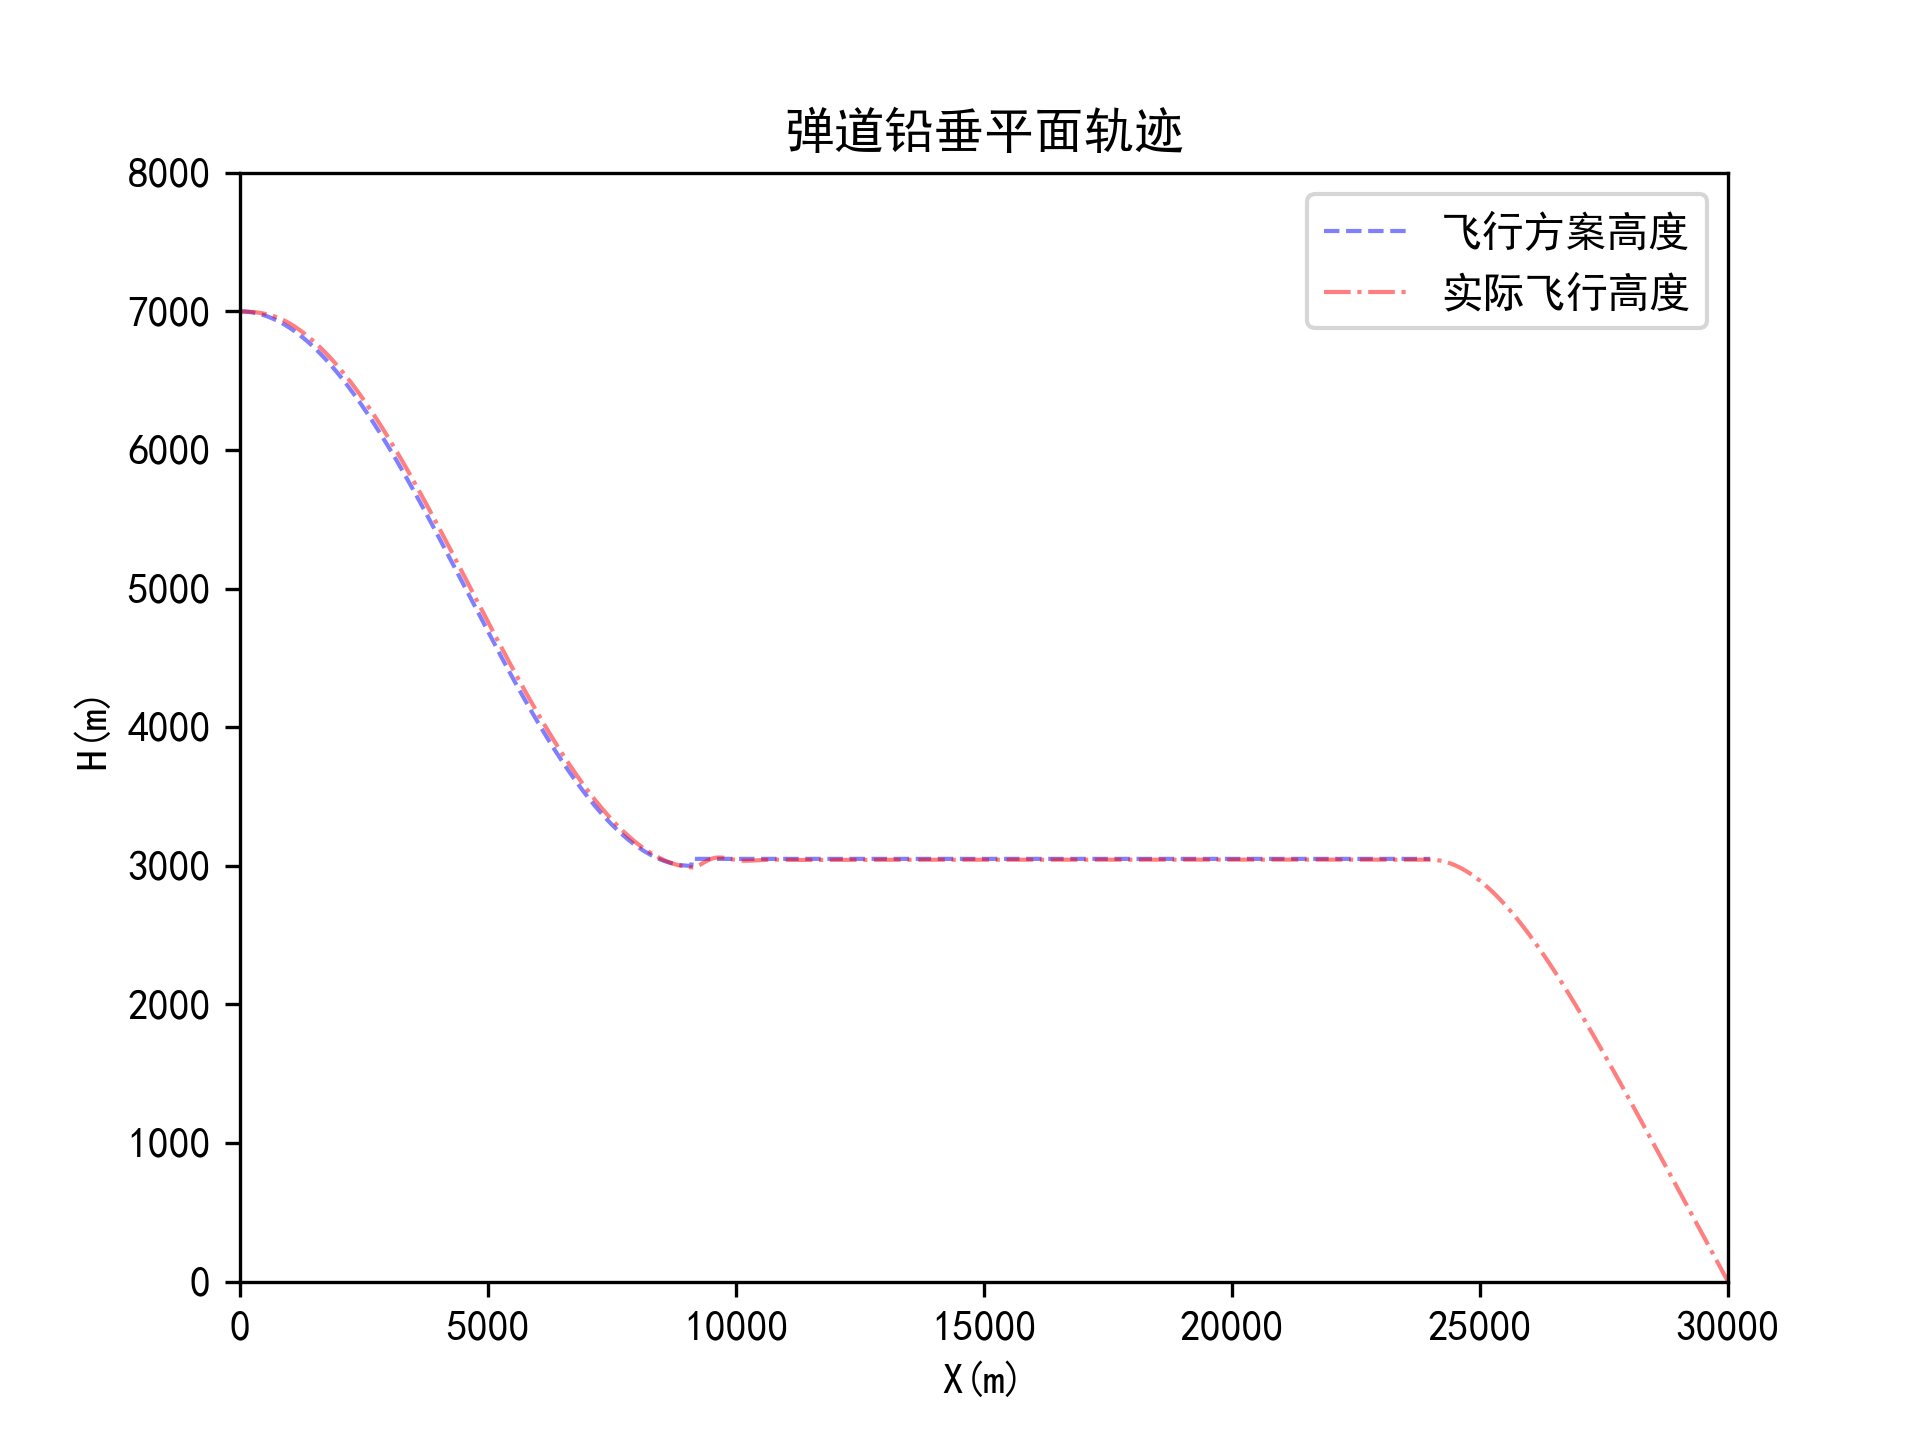
\includegraphics[width=130mm]{../img/飞行轨迹.png}
    \caption{导弹飞行轨迹图}
\end{figure}

\begin{figure}[H]
    \centering
    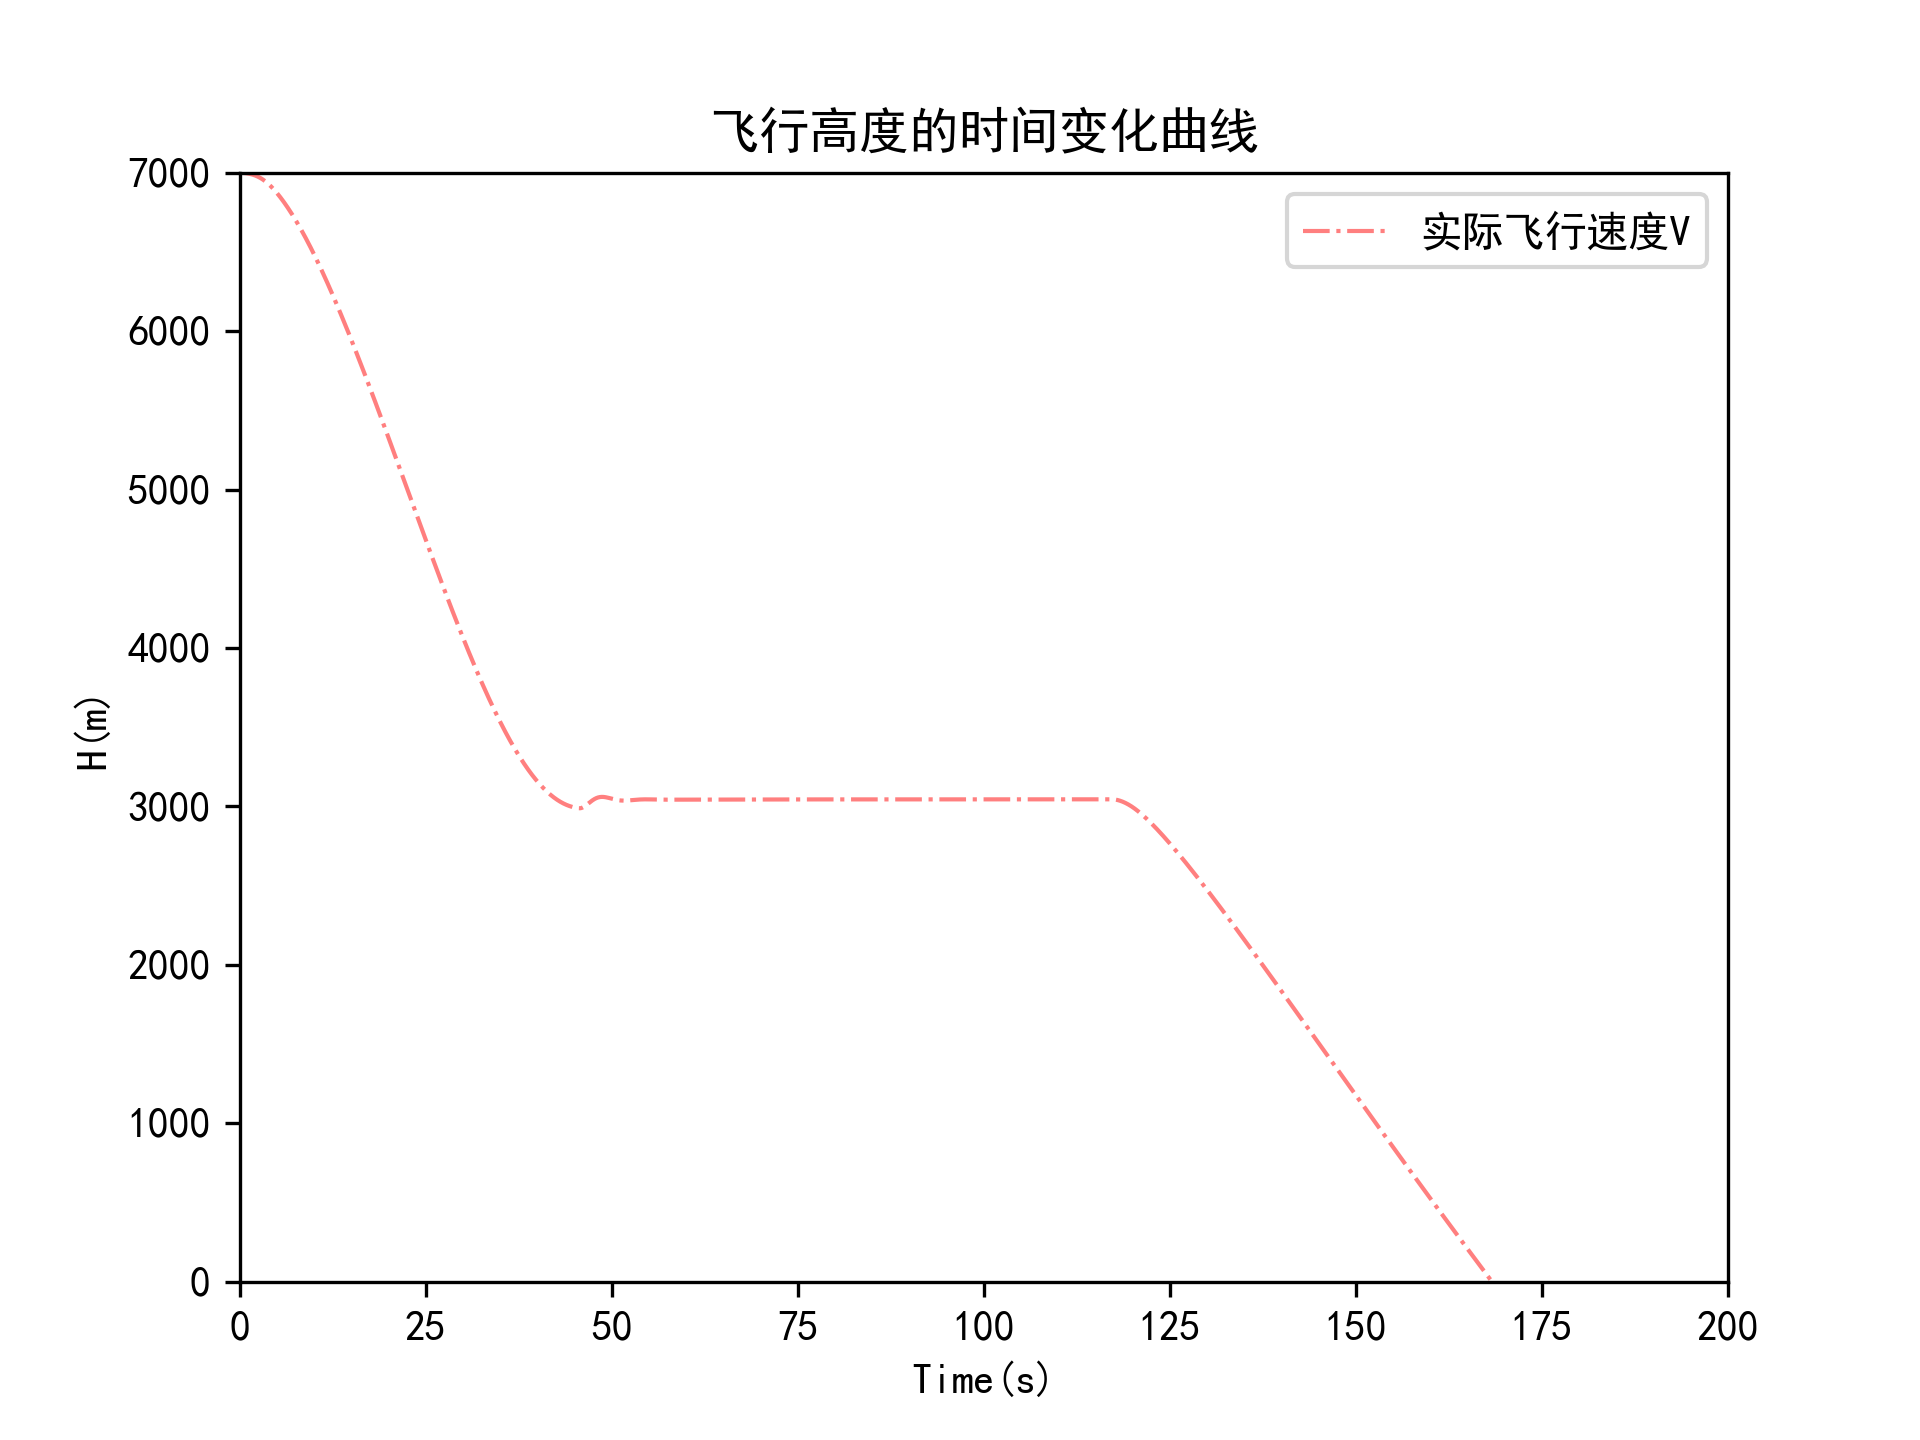
\includegraphics[width=130mm]{../img/飞行高度.png}
    \caption{导弹飞行高度的时间曲线图}
\end{figure}
\begin{figure}[H]
    \centering
    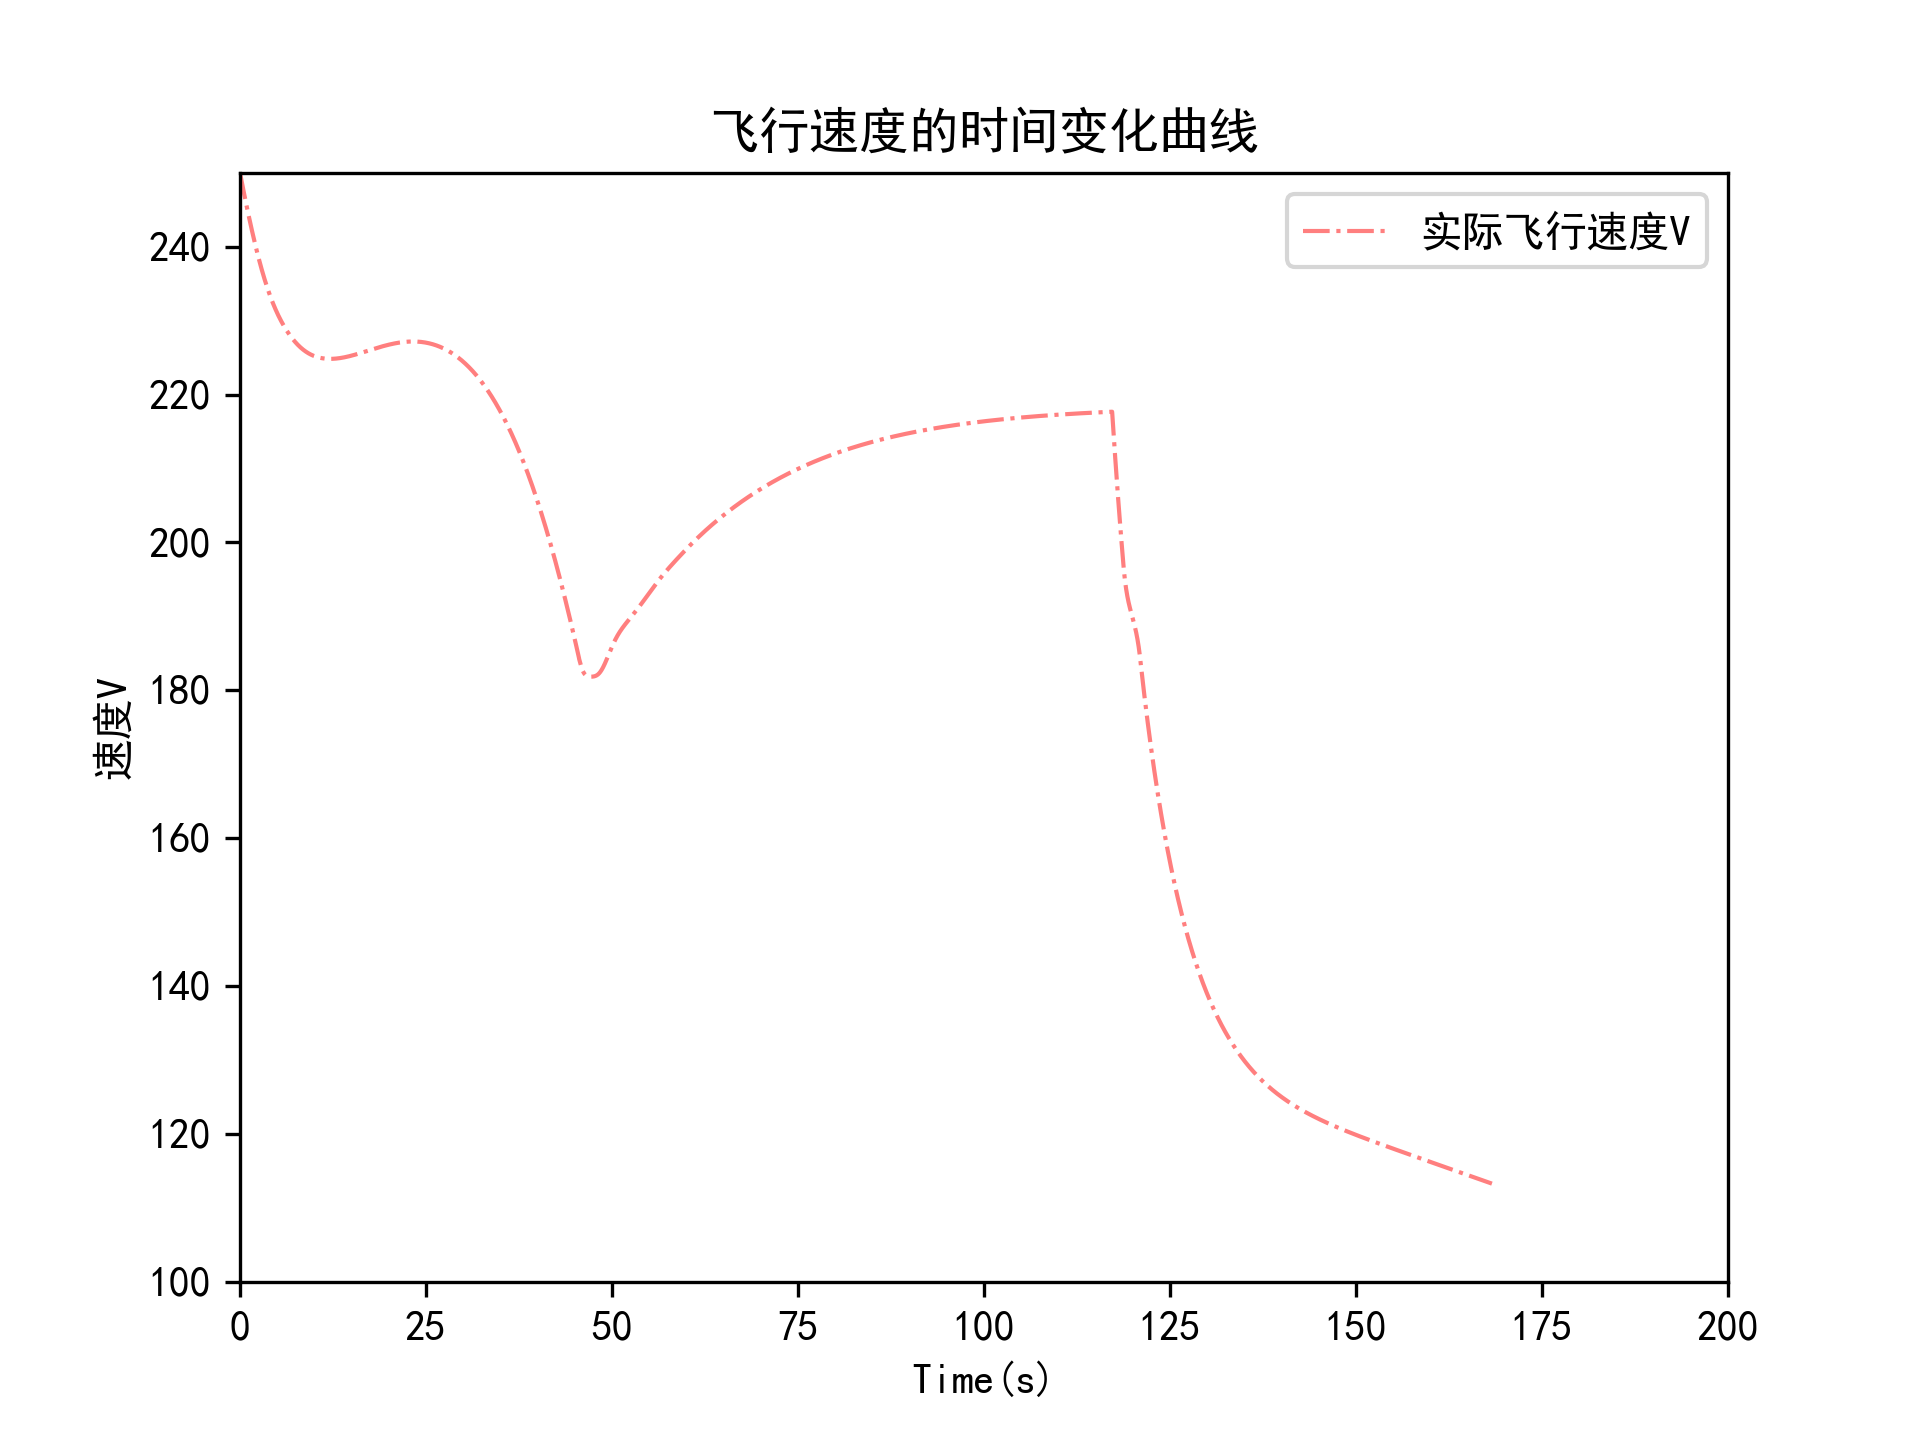
\includegraphics[width=130mm]{../img/飞行速度.png}
    \caption{导弹飞行速度的时间曲线图}
\end{figure}
\begin{figure}[H]
    \centering
    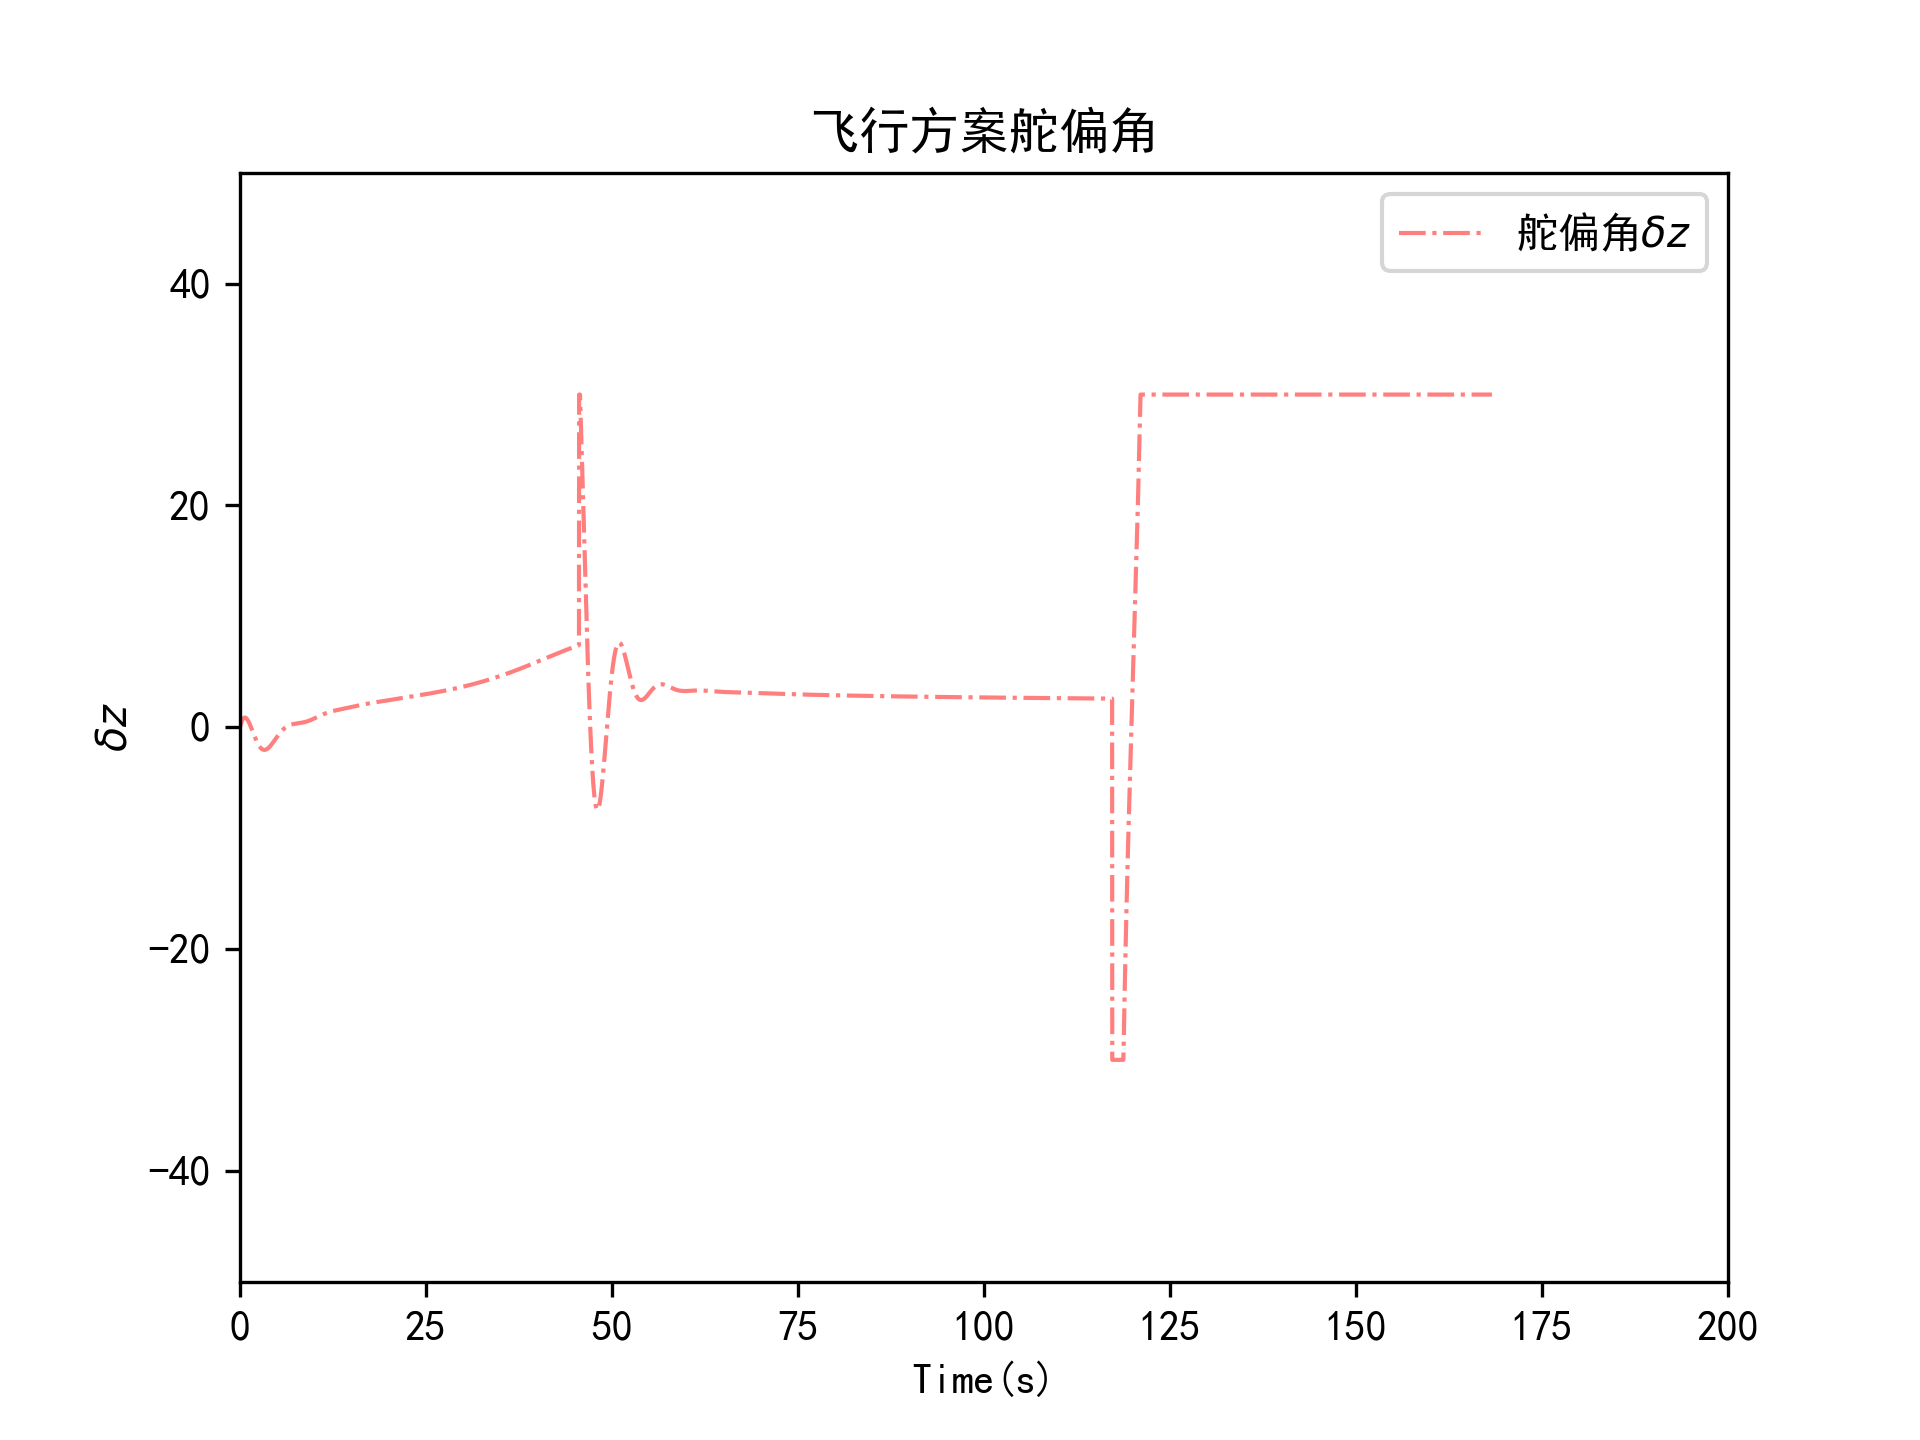
\includegraphics[width=130mm]{../img/飞行舵偏角.png}
    \caption{导弹飞行舵偏角的时间曲线图}
\end{figure}
\begin{figure}[H]
    \centering
    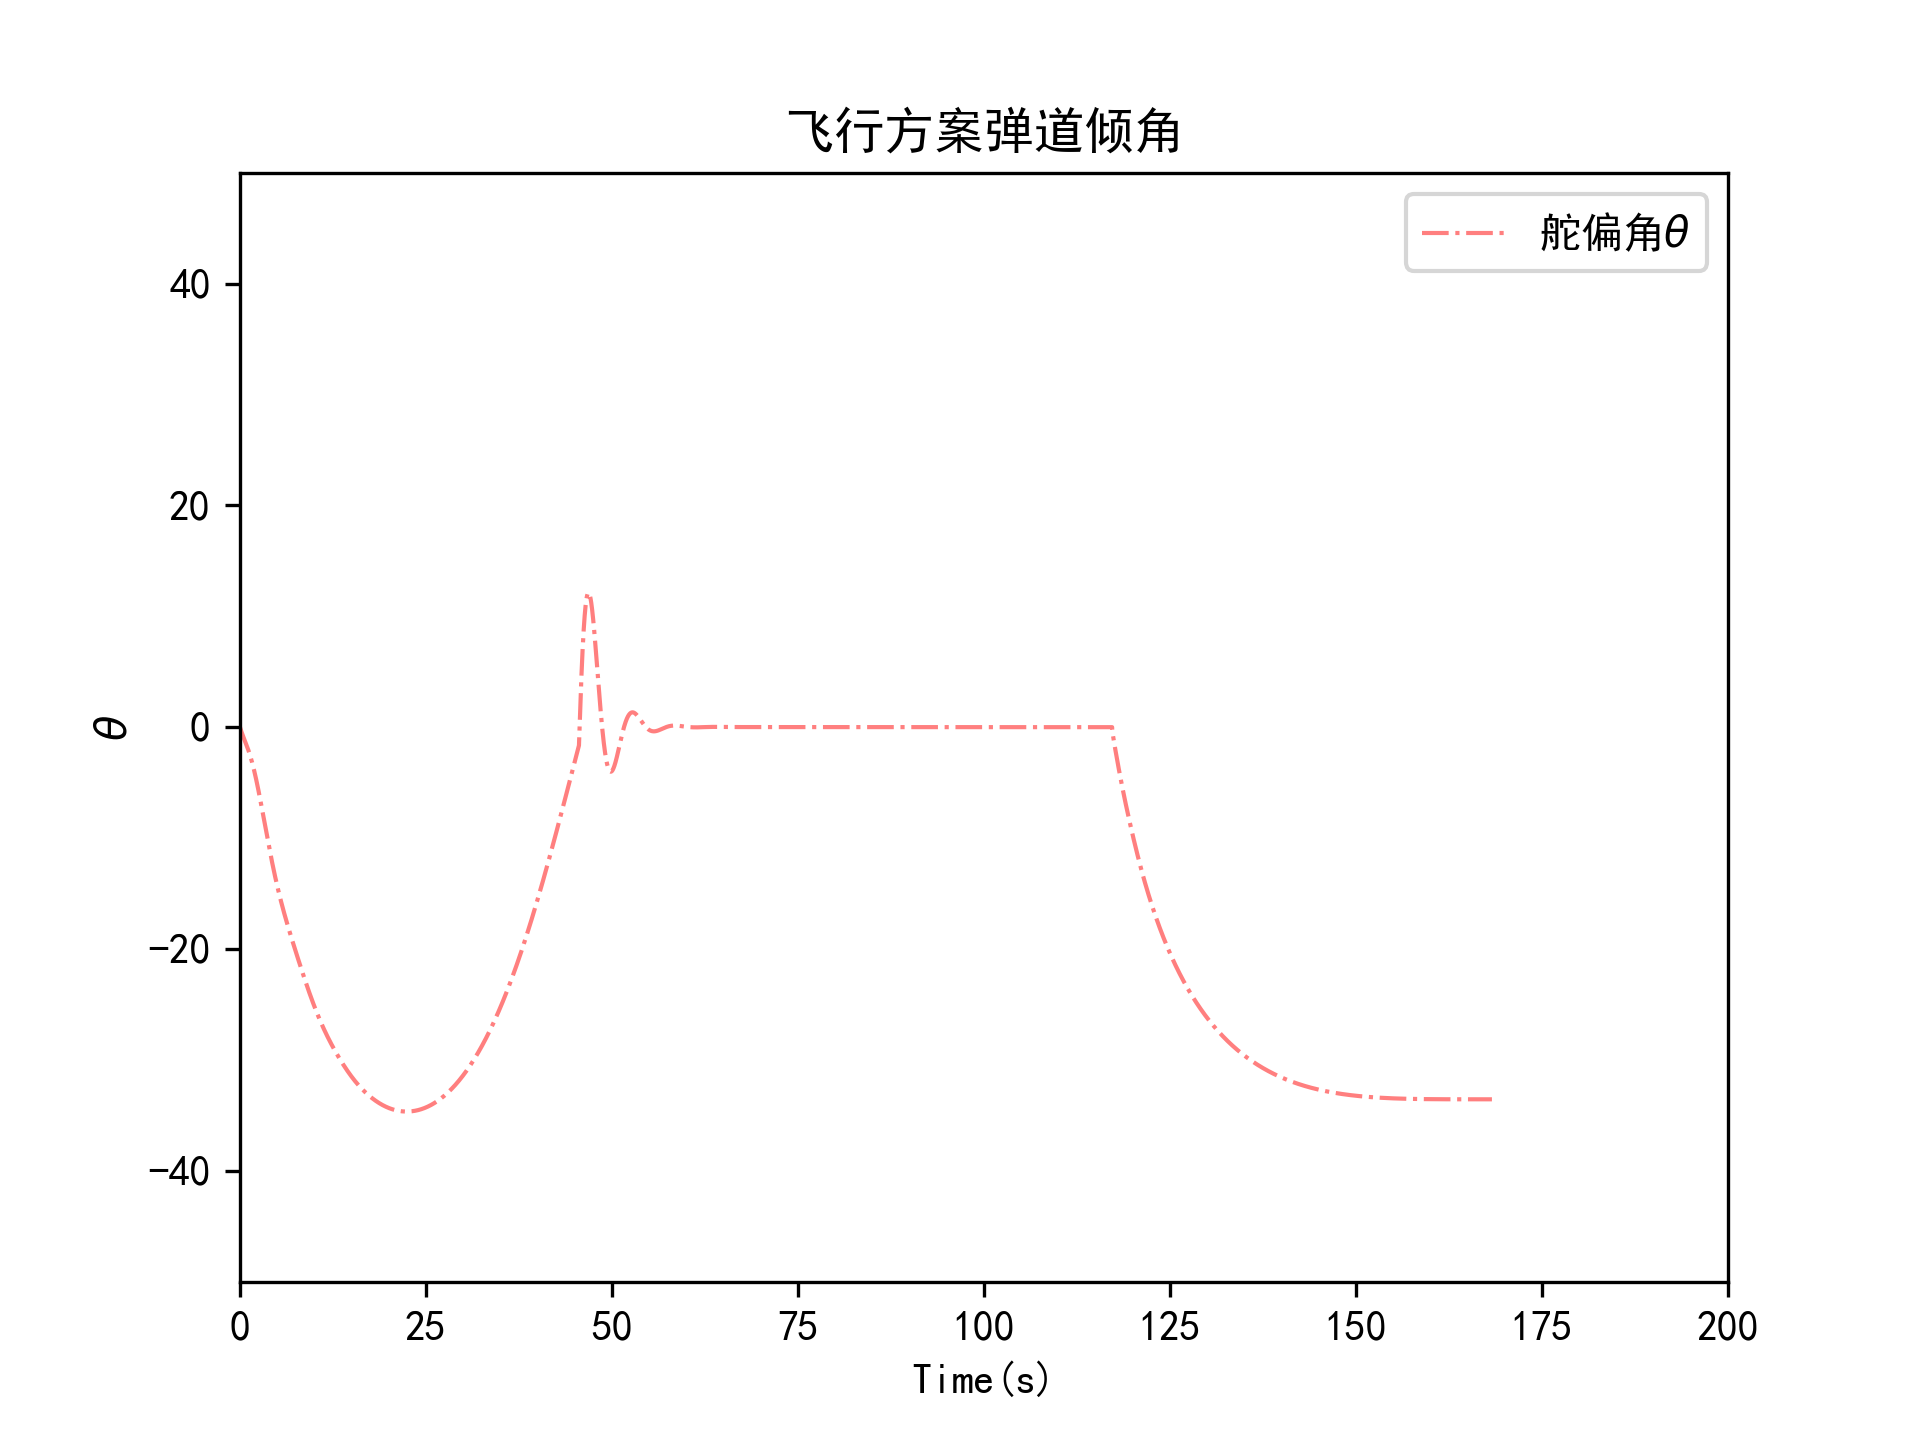
\includegraphics[width=130mm]{../img/飞行弹道倾角.png}
    \caption{导弹飞行弹道倾角的时间曲线图}
\end{figure}

\section*{\zihao{-4} 四、结果分析}

\noindent {\heiti 1.$k_{\varphi}$的影响:}
\begin{figure}[H]
    \centering
    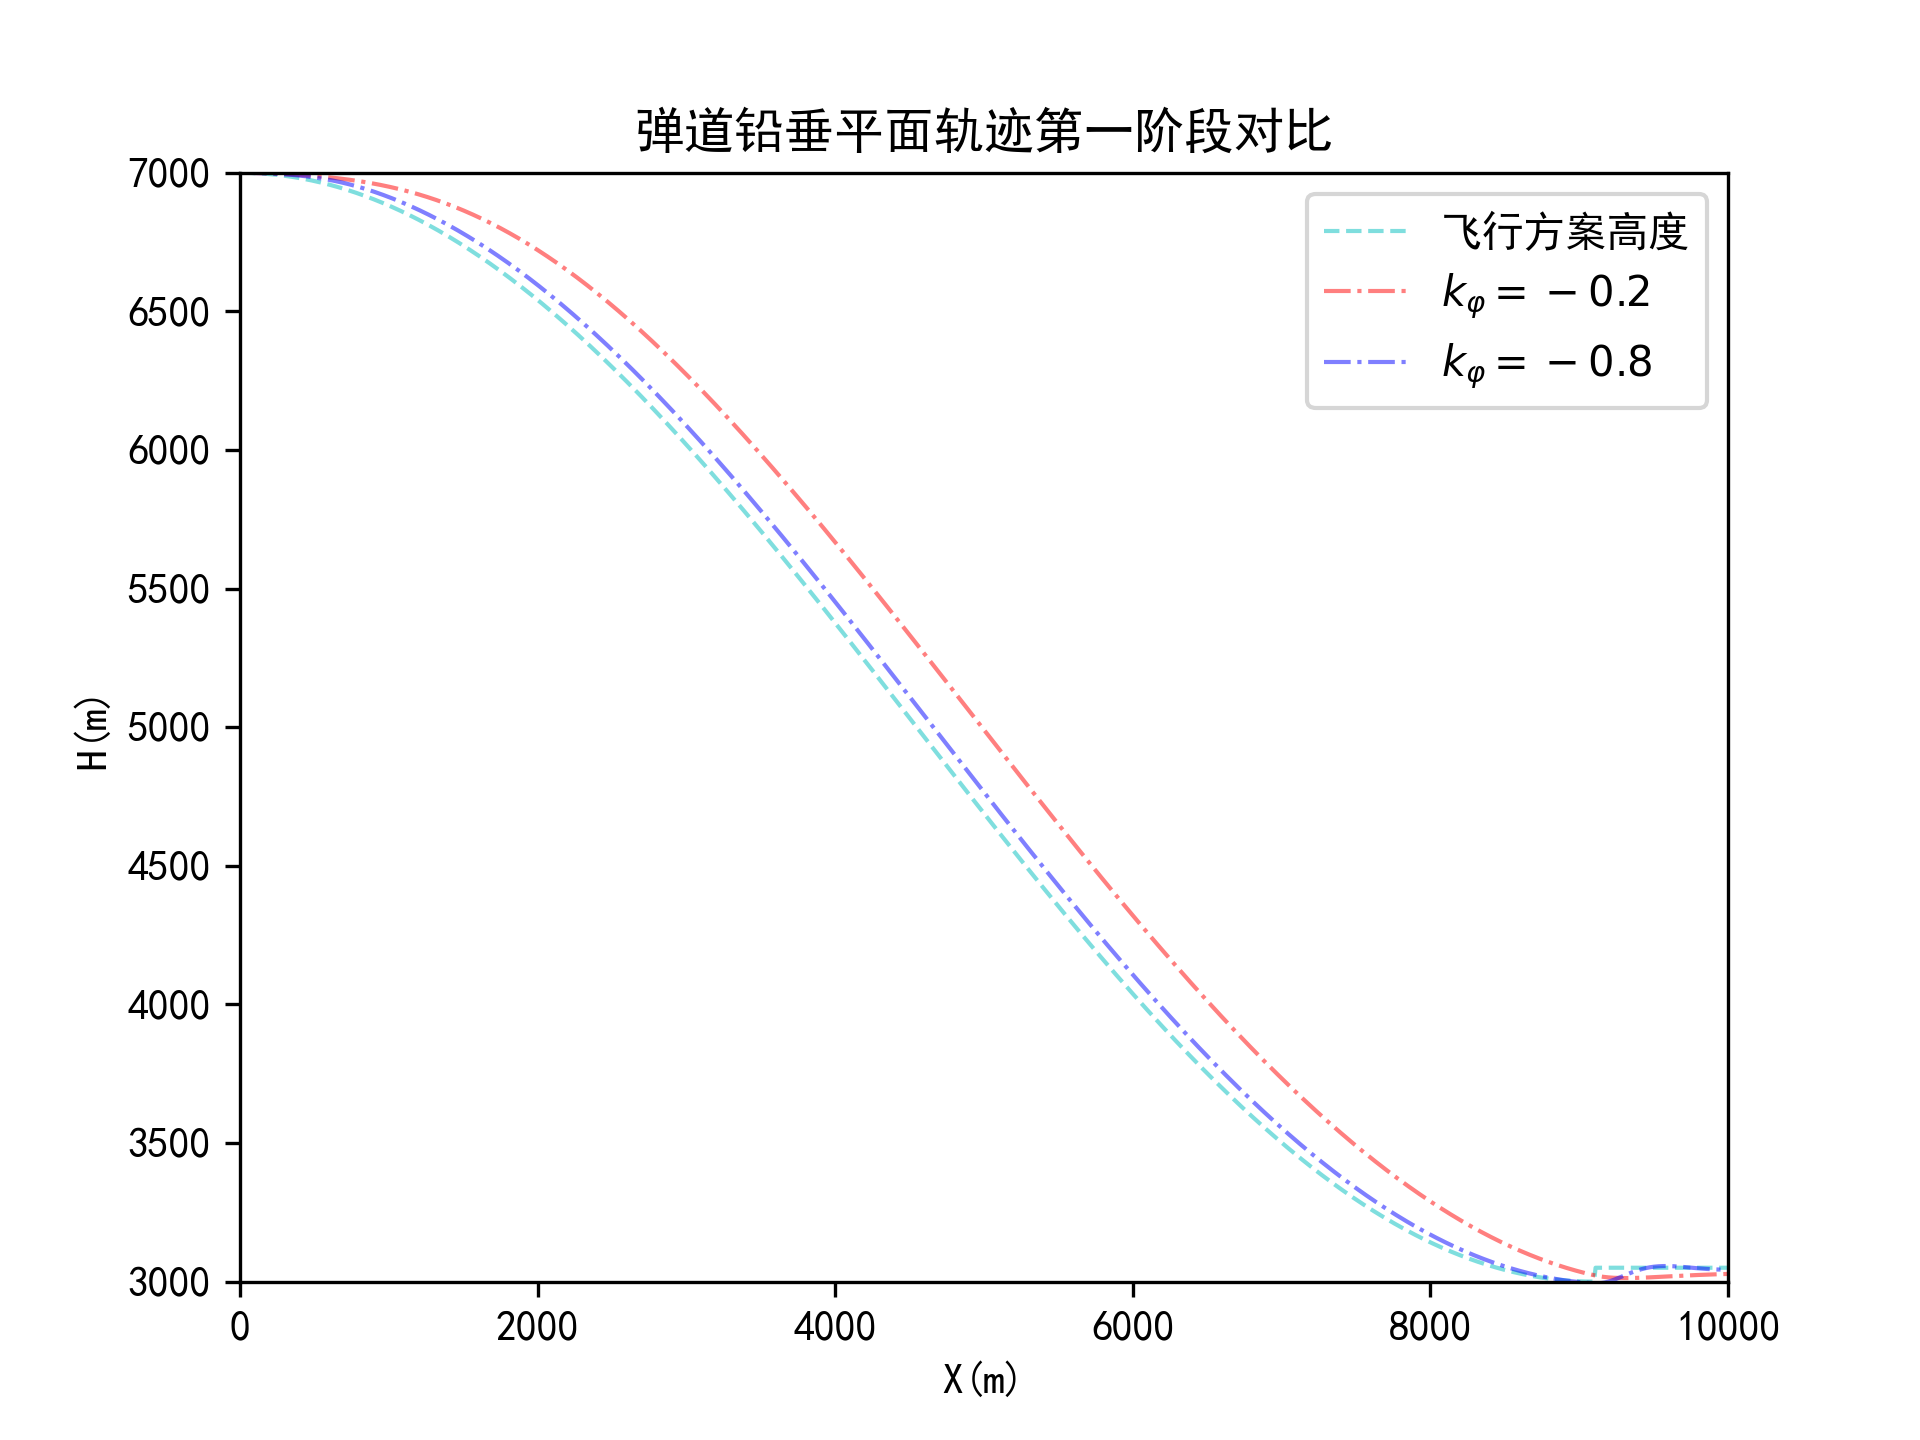
\includegraphics[width=70mm]{../img/飞行轨迹2.png}
    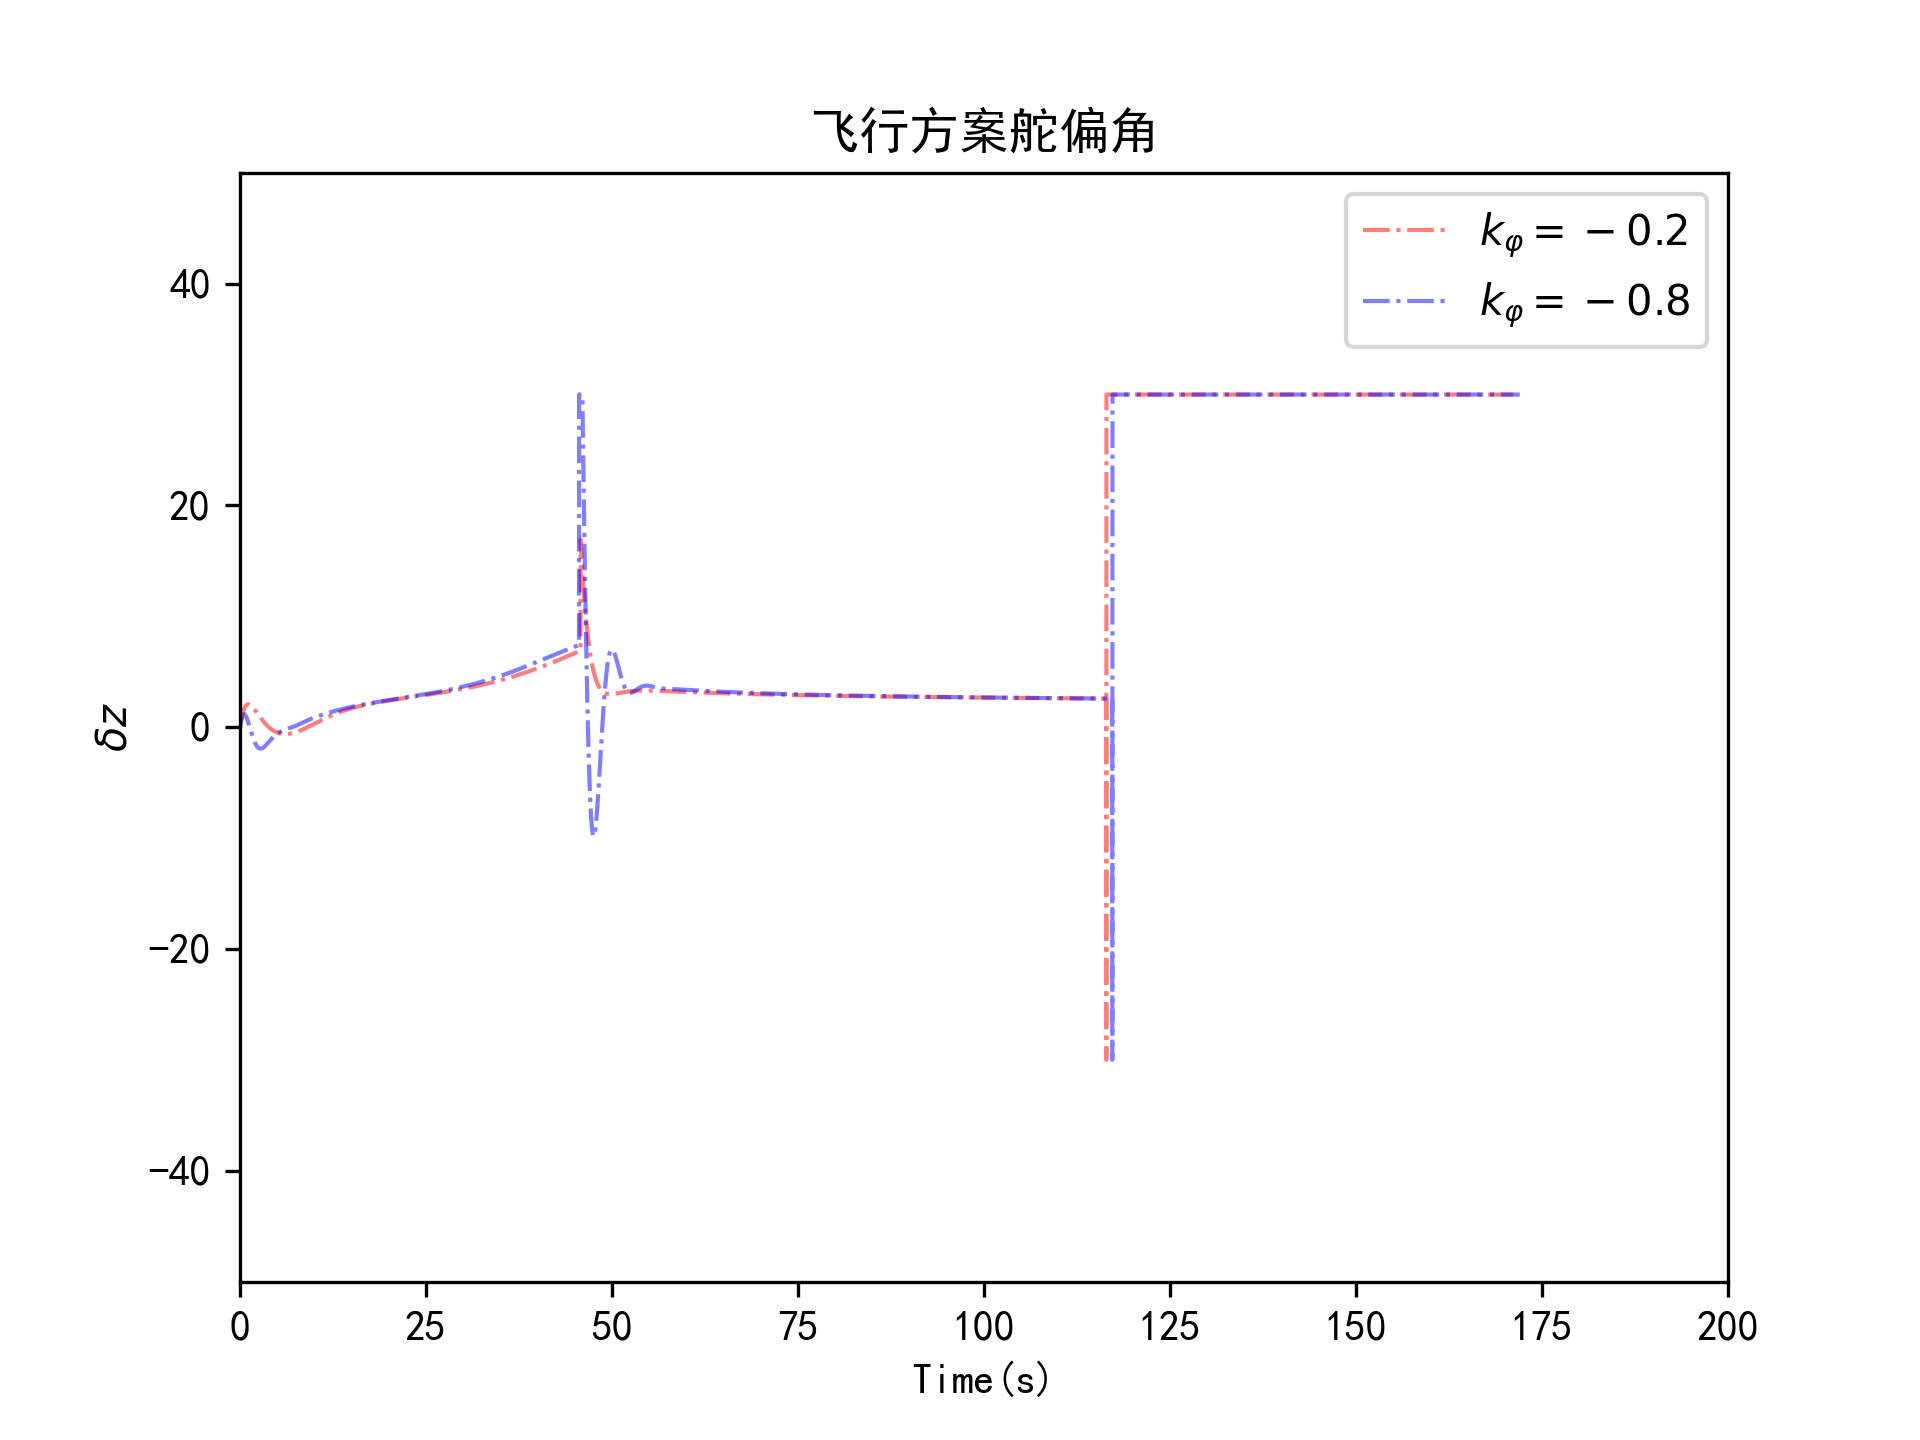
\includegraphics[width=70mm]{../img/飞行舵偏角2.png}
    \caption{$K_{\varphi}$大小对导弹飞行弹道和舵偏角的影响}\label{fig:k1}
\end{figure}

如图~\ref{fig:k1}所示,$K_{\varphi}$是理想控制方程的放大系数,$K_{\varphi}$绝对值越大,导弹越快地恢复到预定的飞行方案。

\noindent {\heiti 2.$\dot{K}_{\varphi}$的影响:}
\begin{figure}[H]
    \centering
    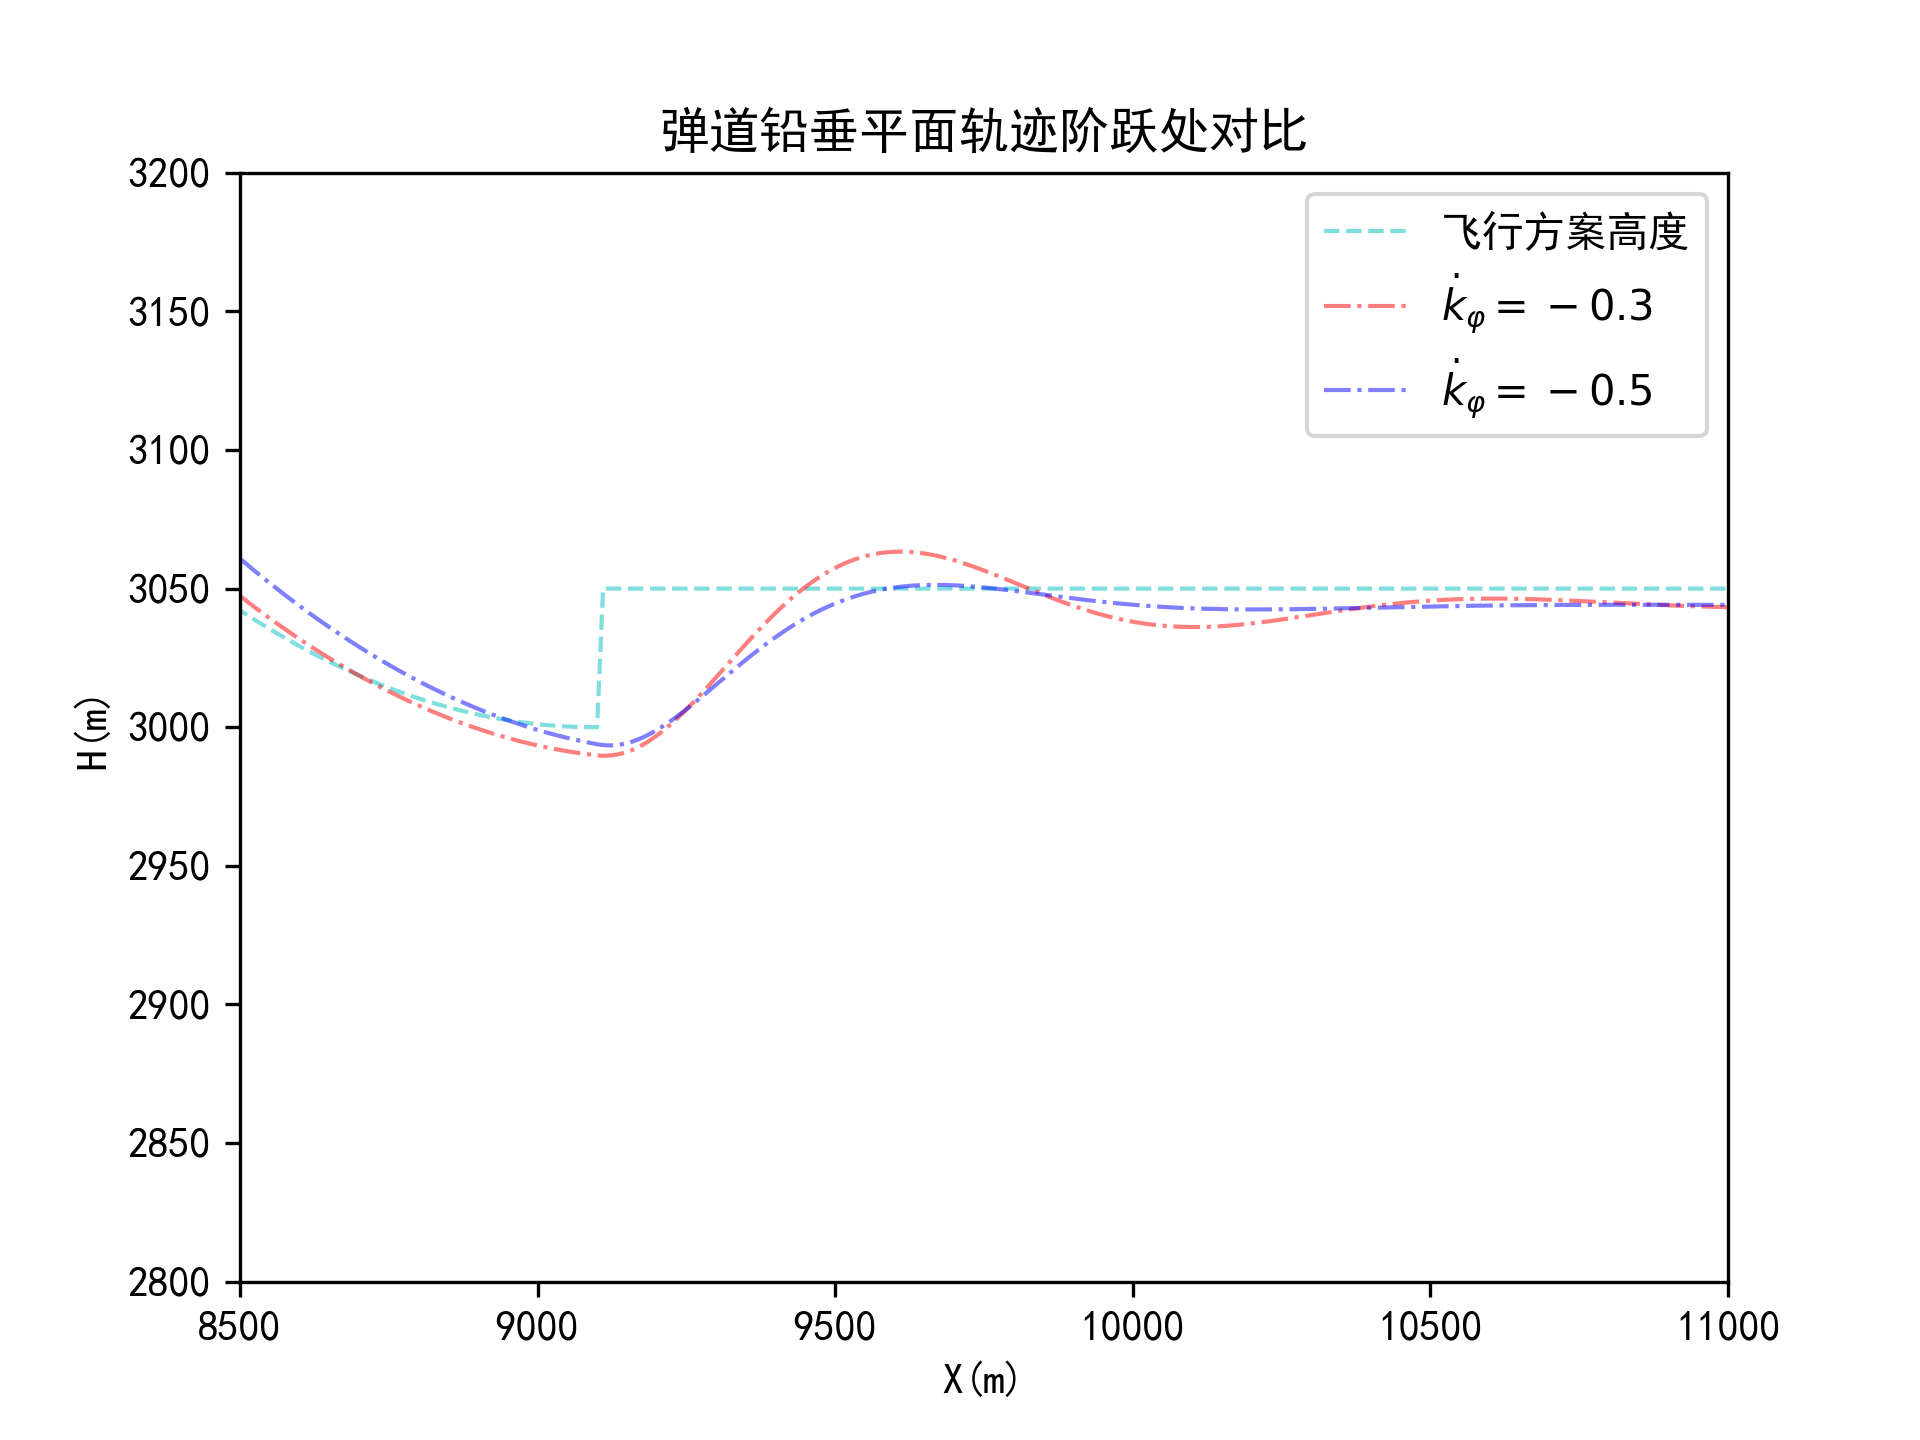
\includegraphics[width=70mm]{../img/飞行轨迹3.png}
    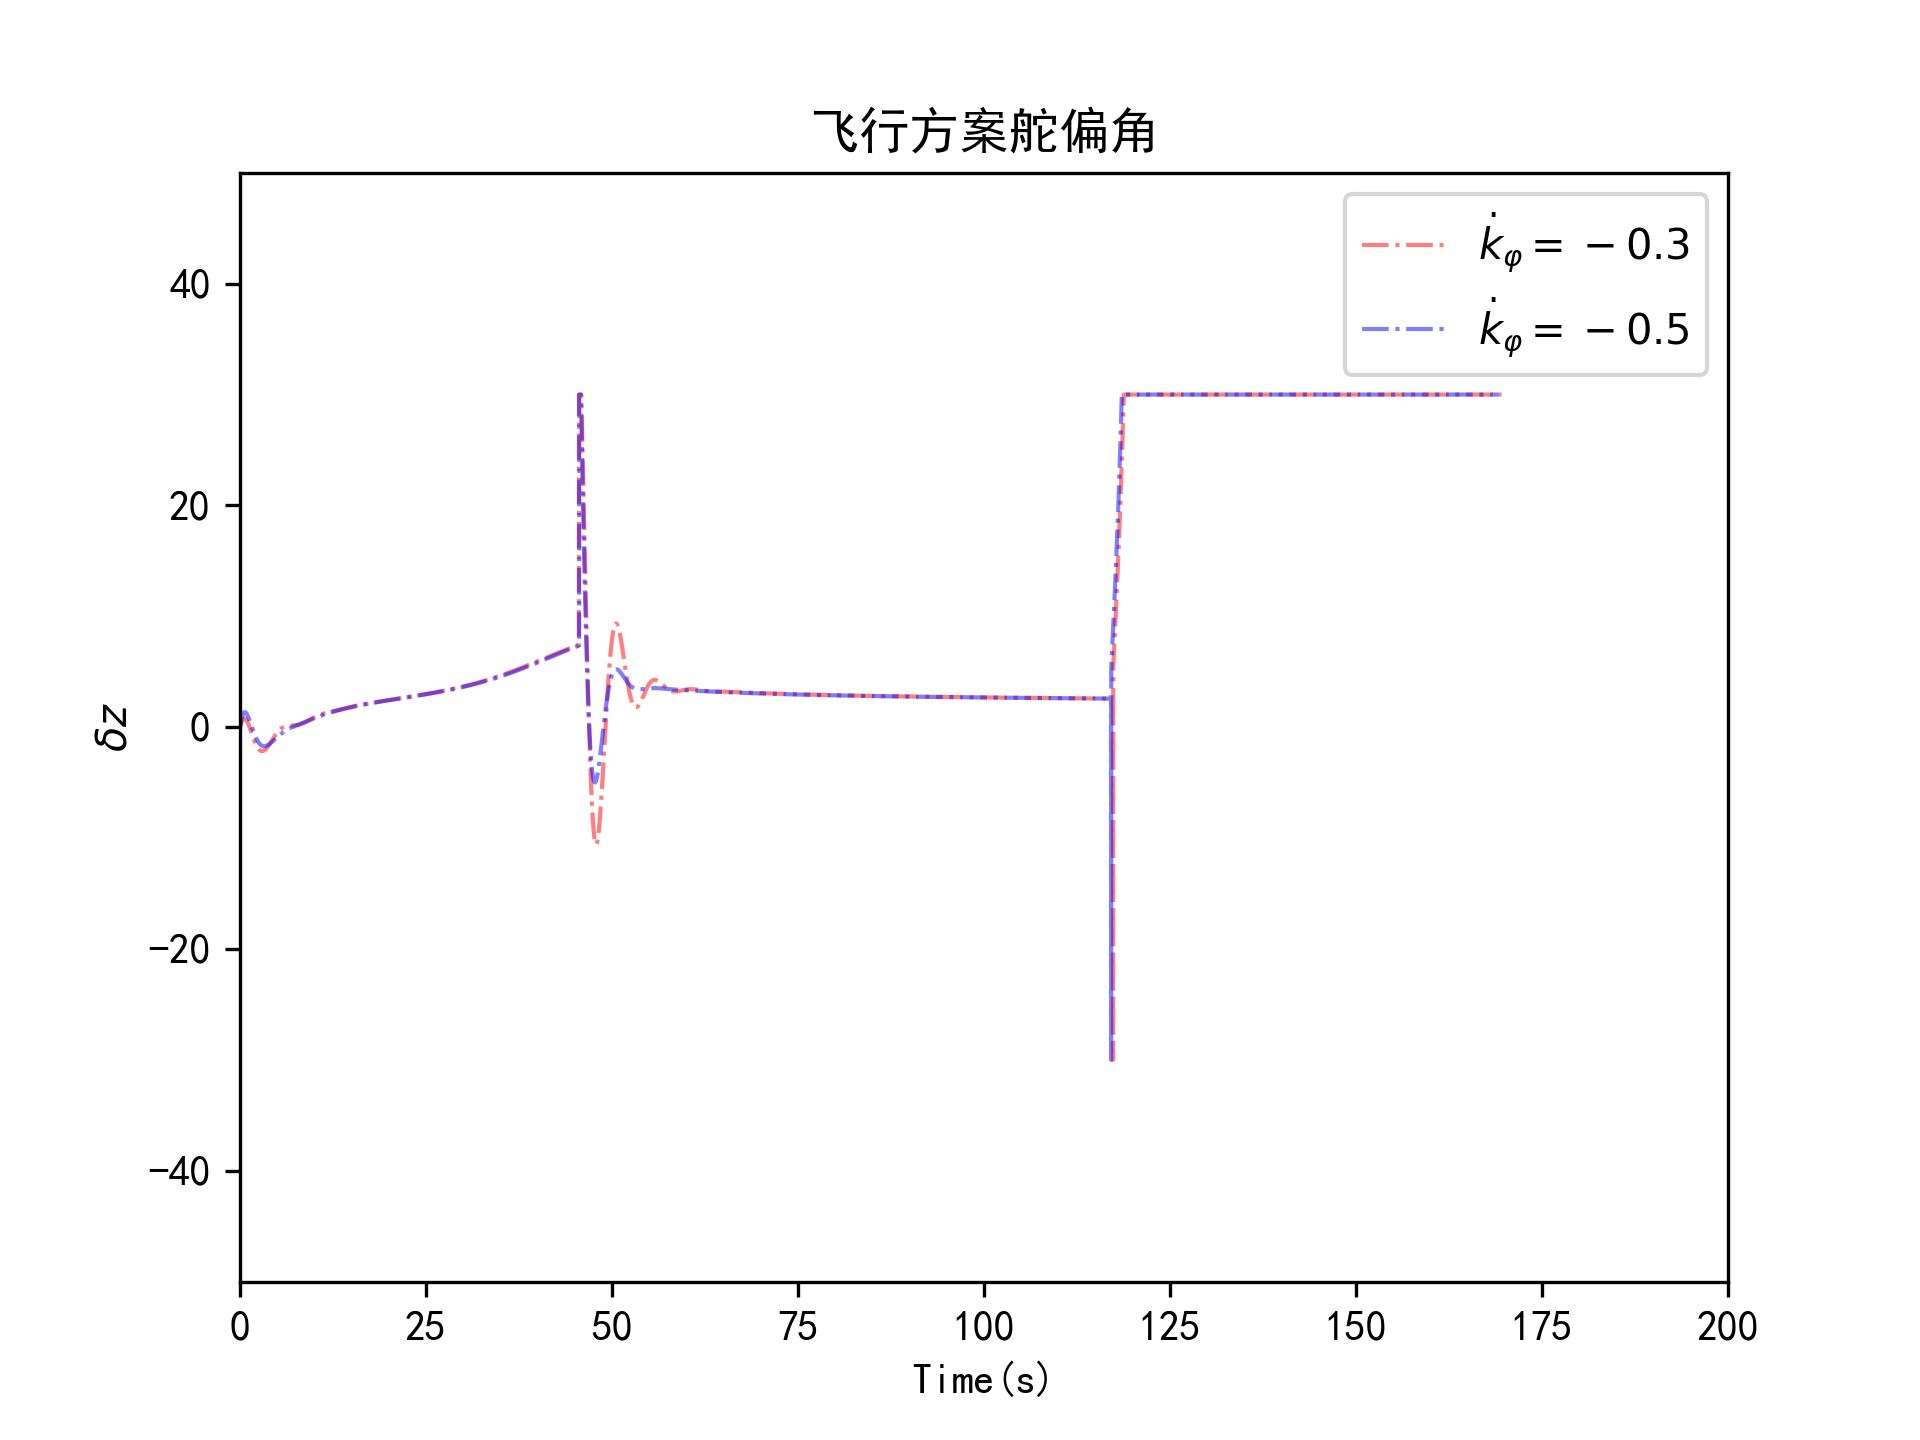
\includegraphics[width=70mm]{../img/飞行舵偏角3.png}
    \caption{$\dot{K}_{\varphi}$大小对导弹飞行弹道和舵偏角的影响}\label{fig:k2}
\end{figure}

如图~\ref{fig:k2}所示,$\dot{K}_{\varphi}$是用于减小超调量的放大系数,起到阻尼作用,$k_{\varphi}$绝对值越大,导弹越快地稳定到预定的飞行方案。


\noindent {\heiti 3.${k}_{3}$的影响:}
\begin{figure}[H]
    \centering
    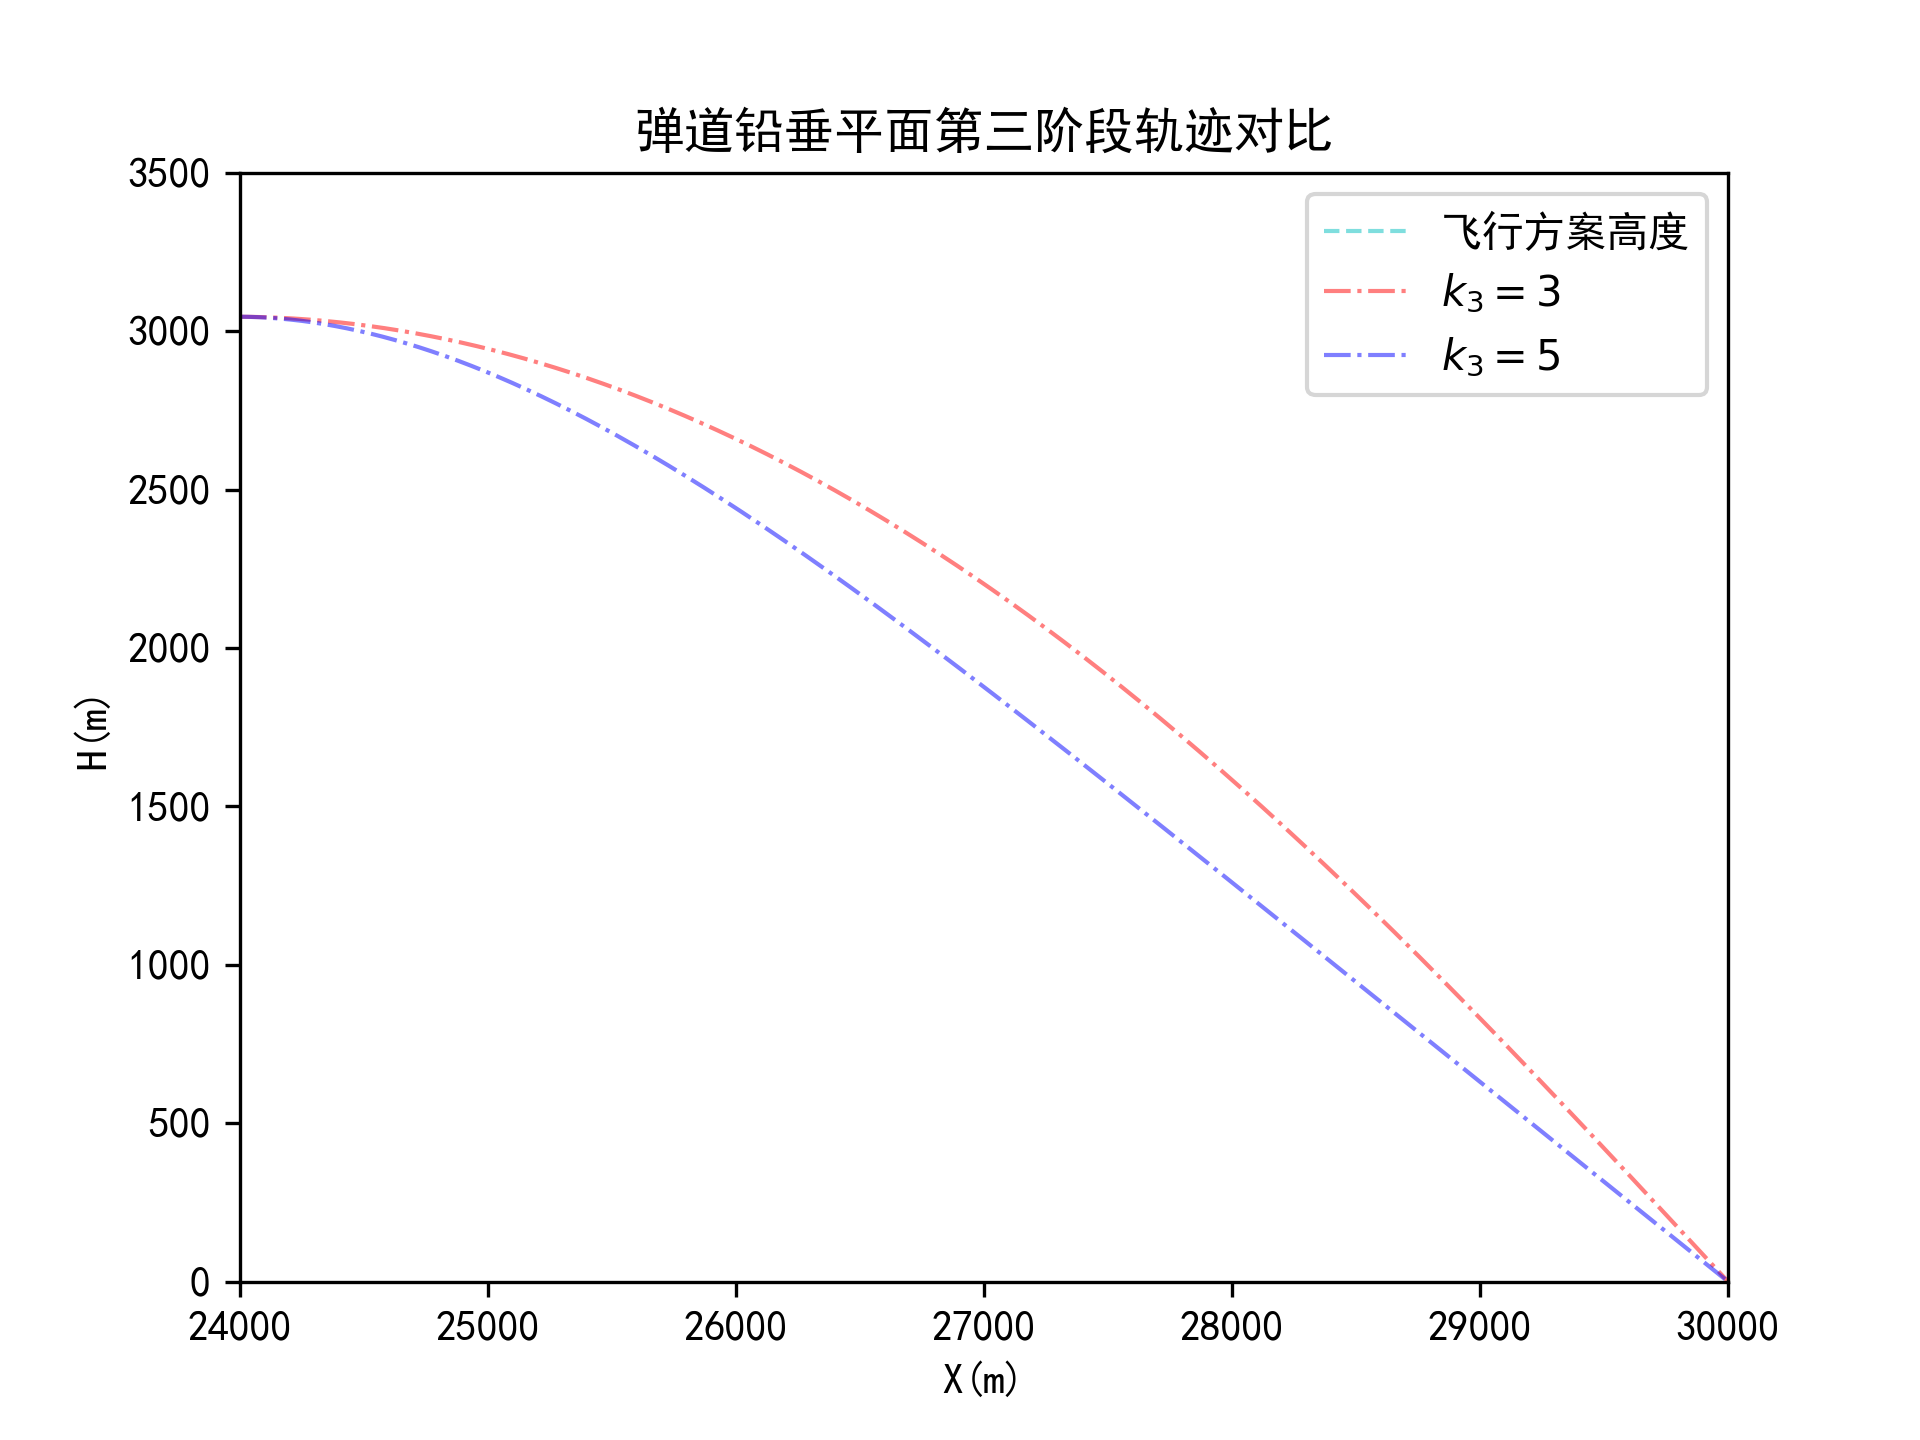
\includegraphics[width=70mm]{../img/飞行轨迹4.png}
    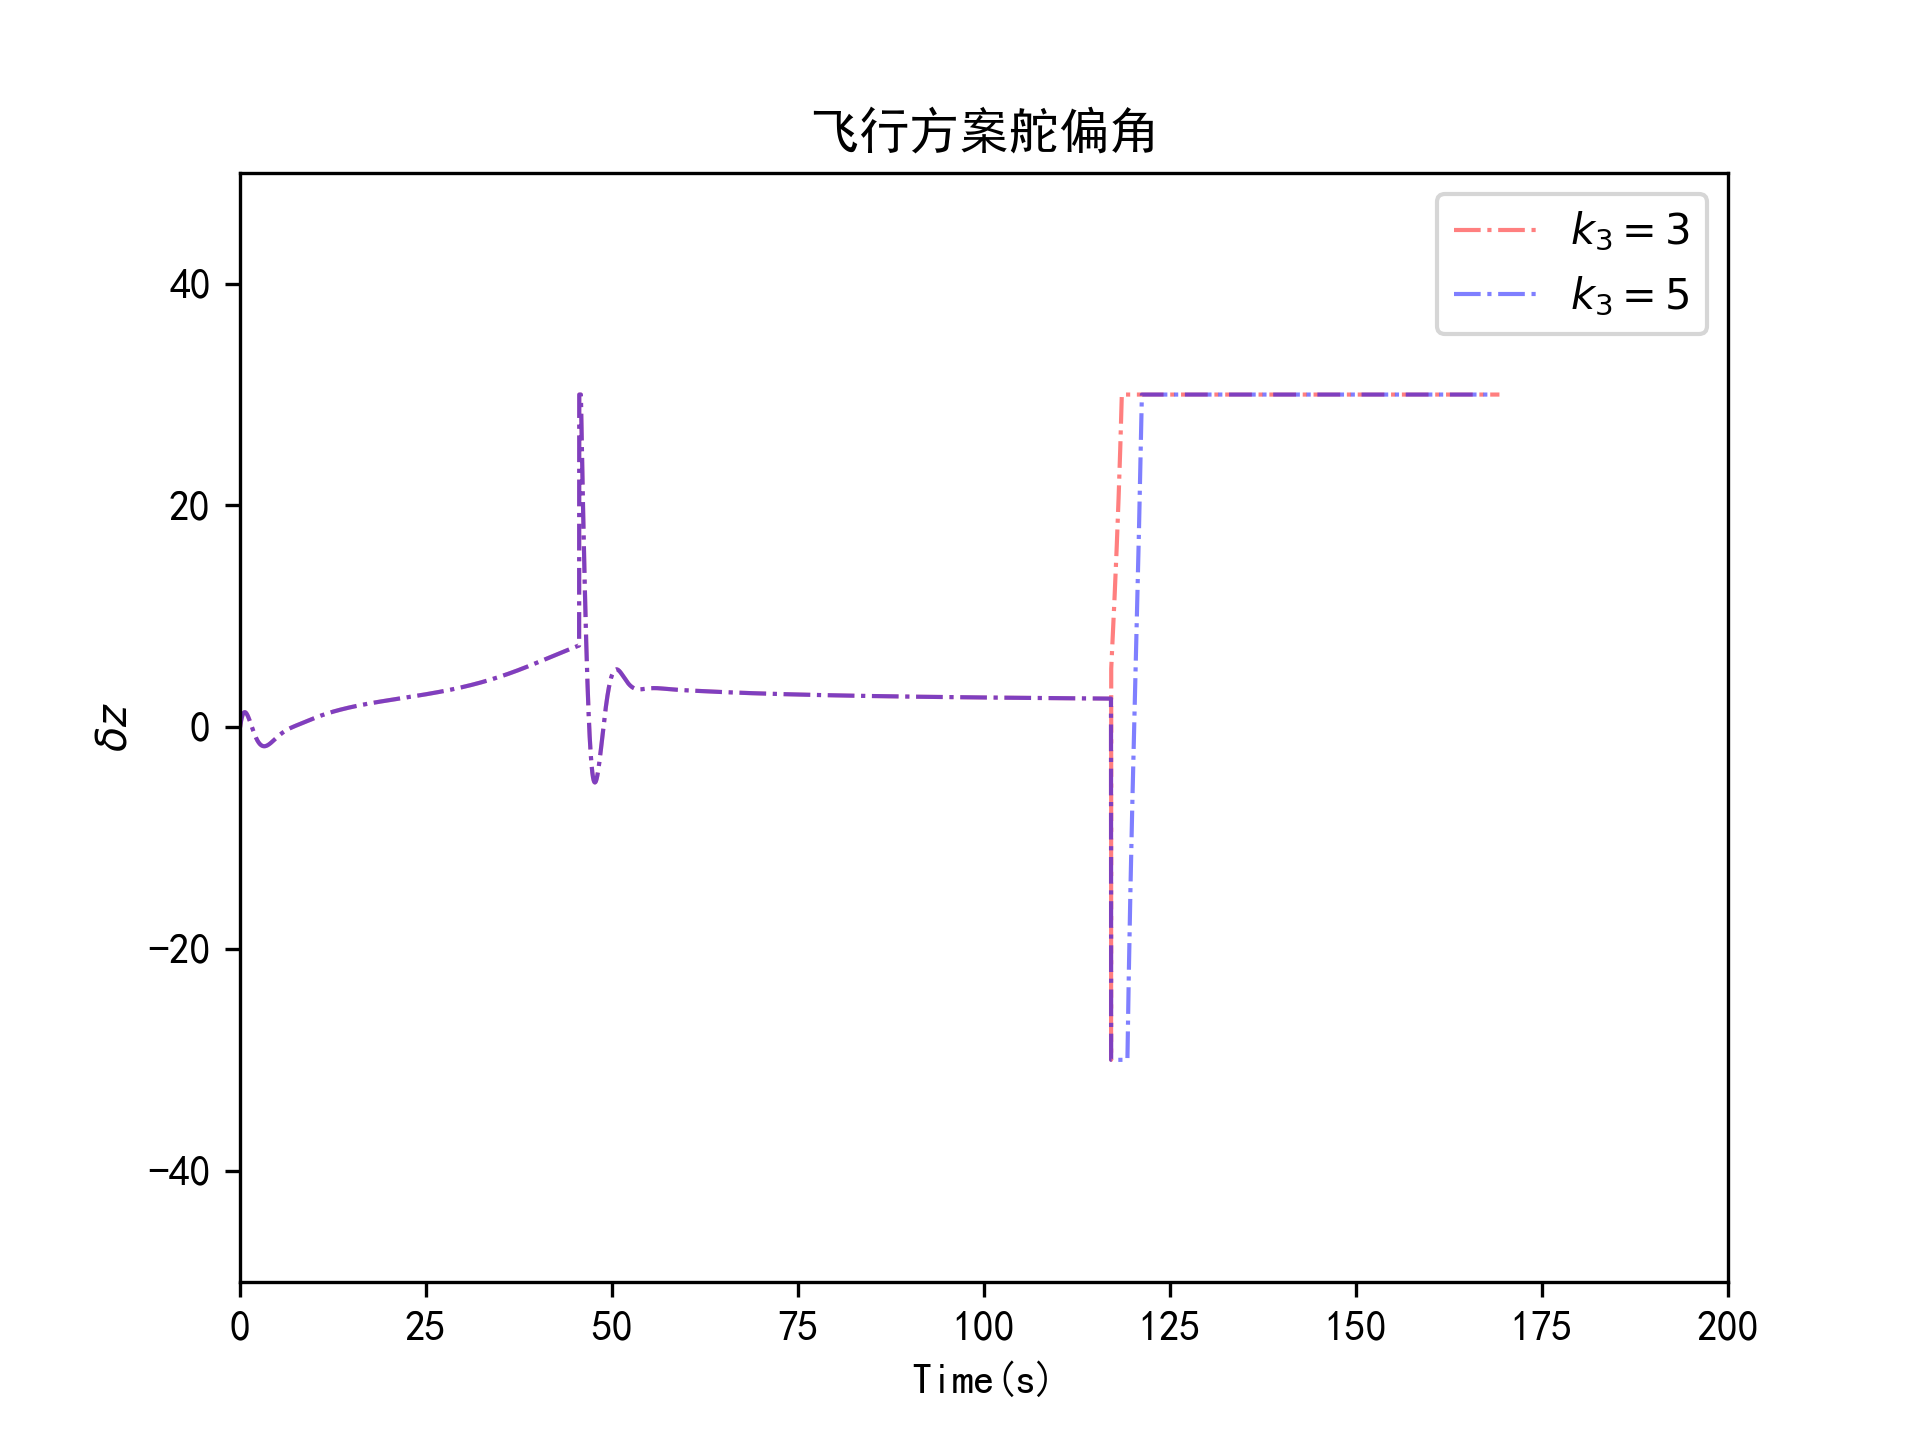
\includegraphics[width=70mm]{../img/飞行舵偏角4.png}
    \caption{$k_3$大小对导弹飞行弹道和舵偏角的影响}\label{fig:k3}
\end{figure}
如图~\ref{fig:k3}所示,$K_{3}$是比例导引法的比例系数,$K_3$越大,后期弹道约平直。
~\\
~\\

\bf 注:第三阶段的舵偏角由于使用显式的Euler法计算,结果有一定的发散。
\clearpage
\lstinputlisting[
    style       =   Python,
    caption     =   {\bf main.py},
    label       =   {main.py}
]{../code/main.py}



\clearpage
\lstinputlisting[
    style       =   Python,
    caption     =   {\bf comparis.py},
    label       =   {comparison.py}
]{../code/comparison.py}


\end{document}
